% Modelo para monografia de final de curso, em conformidade
% com normas da ABNT implementadas pelo projeto abntex2.
%
% Este arquivo é fortemente baseado em exemplo distribuído no
% mesmo projeto. O projeto abntex2 pode ser acessado pela página
% http://abntex2.googlecode.com/
%
% Este arquivo pode ser rodado tanto com o pdflatex quanto com
% o lualatex.  Como contém referências bibliográficas a serem
% processadas pelo programa bibtex, este programa deve ser
% executado. Em resumo, a ordem de execução deve ser:
% rodar primeiro o pdflatex (ou o lualatex), depois o bibtex e,
% a seguir, o pdflatex (ou o lualatex ) novamente mais duas vezes,
% para assegurar que todas as referências bibliográficas e 
% citações estejam atualizadas.
%
% Para adaptar os textos para uso pessoal, usar os comandos
% imediatamente antes do \begin{document} (iniciando com o
% comando \titulo).  
%
% Este modelo está adaptado para monografias de final de curso
% em matemática da UFRJ, mas, com o uso das variáveis, pode ser
% usado para outros tipos de trabalho (mestrado, doutorado),
% outros cursos, universidades etc.  Caso a adaptação das
% variáveis não seja suficiente, pode-se alterar os comandos
% imprimircapa, imprimirfolhaderosto e imprimiraprovação, 
% fazendo as alterações necessárias.  Como os comandos definidos
% neste texto usam somente LaTeX, a sua adaptação deve ser 
% simples, bastando algum conhecimento de LaTeX.
%
% O restante do preâmbulo provavelmente  não necessitará ser
% alterado, a menos, eventualmente, das opções de chamada da
% classe abntex2, que estão definidas a seguir.
% 
\documentclass[ 
% -- opções da classe memoir que é a classe base da abntex2 --
% tamanho da fonte
12pt,
% capítulos começam em pág ímpar. Insere pág vazia, se preciso
openright,
% para imprimir uma página por folha ou visualização em video 
oneside,
% frente e verso. Margens das pag. ímpares diferem das pares.
%  twoside,
% tamanho do papel. 
a4paper,
% Caio - Ocultando bordas horríveis em hiperligações
hidelinks,
% -- opções da classe abntex2 --
% títulos de capítulos convertidos em letras maiúsculas
%  chapter=TITLE,
% títulos de seções convertidos em letras maiúsculas
%  section=TITLE,
% títulos de subseções convertidos em letras maiúsculas
%  subsection=TITLE,
% títulos de subsubseções convertidos em letras maiúsculas
%  subsubsection=TITLE,
% -- opções do pacote babel --
english,   % idioma adicional para hifenização
portuguese,   % o último idioma é o principal do documento
oldfontcommands,
]{abntex2}

% --------------------------------------------------------------
% --------------------------------------------------------------
% cabeçalho comum para uso com lualatex ou pdflatex
\usepackage{ifluatex}
% opções para uso com o lualatex
\ifluatex
\usepackage{fontspec}
\defaultfontfeatures{Ligatures=TeX}
% o fonte small caps é diferente no latin modern
\fontspec[SmallCapsFont={Latin Modern Roman Caps}]{Latin Modern Roman}
% pacotes da AMS 
\usepackage{amsmath,amsthm} 
% pacote para fonte específico para símbolos matemáticos
\usepackage{unicode-math}
\setmathfont{Latin Modern Math}
% latin modern tem simbolos de mathbb muito feios.
%  Trocar o fonte para estes simbolos.
\setmathfont[range=\mathbb]{Tex Gyre Pagella Math}
% opções para uso com o pdflatex
\else
\usepackage[utf8x]{inputenc}
\usepackage[T1]{fontenc}
\usepackage{lmodern}
\usepackage{etoolbox}
% pacotes da AMS 
\usepackage{amsmath,amssymb,amsthm} 
% Mapear caracteres especiais no PDF
\usepackage{cmap}
\fi

% pacotes usados tanto pelo lualatex quanto pelo pdflatex
\usepackage{lastpage}    % Usado pela Ficha catalográfica
\usepackage{indentfirst} % Indenta primeiro parágrafo 
\usepackage{color}       % Controle das cores
\usepackage{graphicx}    % Inclusão de gráficos
\usepackage{wrapfig}    % gráficos ao redor do texto
% pacote para ajustar os fontes em cada linha de forma a
% respeitar as margens
\usepackage{microtype}
% permite a gravação de texto em um arquivo indicado a partir
% deste arquivo.  Está sendo usado para criar o arquivo .bib
% com conteúdo definido neste arquivo, evitando a edição 
% de um arquivo .bib somente para a bibliografia
\usepackage{filecontents}

% Caio - preciso de tabelas longas
\usepackage{longtable}
% Caio - corrigindo espaçamento conforme http://tex.stackexchange.com/questions/5683/how-to-remove-top-and-bottom-whitespace-of-longtable
\setlength{\LTpost}{0pt}
\setlength{\LTpre}{0pt}

% Caio - preciso de plotagens
\usepackage{pgfplots}
\pgfplotsset{compat=1.8}

% Caio - adicionando o pacote hyperref
\usepackage{hyperref}

\hypersetup{
	%pagebackref=true,
	pdftitle={Usando o Trem Metropolitano da CPTM como fio-condutor para abordar questões territoriais na Grande São Paulo}, 
	pdfauthor={Caio César C. Ortega},
	pdfsubject={Território e sociedade},
	colorlinks=false,      		% false: boxed links; true: colored links
	linkcolor=blue,          	% color of internal links
	citecolor=blue,        		% color of links to bibliography
	filecolor=magenta,      	% color of file links
	urlcolor=blue,
	bookmarksdepth=4
}

% Caio - separação silábica
%\hyphenation{}

% Caio - citações mais poderosas
%\usepackage[autostyle]{csquotes}

%-----------------------------------------------------------
%-----------------------------------------------------------
% Caio - habilitar glossário
\usepackage{glossaries}
\makeglossaries

% \newglossaryentry{ex}{name={sample},description={an example}}
\newglossaryentry{abl}{
	name={ABL},
	description={Área Bruta Locável}
}

\newglossaryentry{auj}{
	name={AUJ},
	description={Aglomeração Urbana de Jundiaí}
}

\newglossaryentry{bbtt}{
	name={Benfica BBTT},
	description={Benfica Barueri Transporte e Turismo Ltda}
}

\newglossaryentry{cptm}{
	name={CPTM},
	description={Companhia Paulista de Trens Metropolitanos}
}

\newglossaryentry{cmsp}{
	name={CMSP},
	description={Companhia do Metropolitano de São Paulo}
}

\newglossaryentry{ett}{
	name={ETT},
	description={Empresa de Transportes e Turismo Carapicuíba}
}

\newglossaryentry{emtu}{
	name={EMTU},
	description={Empresa Metropolitana de Transportes Urbanos de São Paulo S.A}
}

\newglossaryentry{emplasa}{
	name={Emplasa},
	description={Empresa Paulista de Planejamento Metropolitano S/A}
}

\newglossaryentry{luos}{
	name={LUOS},
	description={Lei de Uso de Ocupação do Solo}
}

\newglossaryentry{mdu}{
	name={MDU},
	description={Média por Dia Útil}
}

\newglossaryentry{ouc}{
	name={OUC},
	description={Operação Urbana Consorciada}
}


\newglossaryentry{pl}{
	name={PL},
	description={Projeto de Lei}
}


\newglossaryentry{rmsp}{
	name={RMSP},
	description={Região Metropolitana de São Paulo}
}

\newglossaryentry{smdu}{
	name={SMDU},
	description={Secretaria Municipal de Desenvolvimento Urbano da Prefeitura de São Paulo}
}

%-----------------------------------------------------------
%-----------------------------------------------------------
% Comandos para definir ambientes tipo teorema em português 
\newtheorem{meuteorema}{Teorema}[chapter]
\newtheorem{meuaxioma}{Axioma}[chapter]
\newtheorem{meucorolario}{Corolário}[chapter]
\newtheorem{meulema}{Lema}[chapter]
\newtheorem{minhaproposicao}{Proposição}[chapter]
\newtheorem{minhadefinicao}{Definição}[chapter]
\newtheorem{meuexemplo}{Exemplo}[chapter]
\newtheorem{minhaobservacao}{Observação}[chapter]
%-----------------------------------------------------------
%-----------------------------------------------------------
% Pacotes de citações
\usepackage[brazilian,hyperpageref]{backref}
\usepackage[alf]{abntex2cite}   % Citações padrão ABNT
%\usepackage[num]{abntex2cite}  % Citações numéricas
% --- 
% Configurações do pacote backref
% Usado sem a opção hyperpageref de backref
\renewcommand{\backrefpagesname}{Citado na(s) página(s):~}
% Texto padrão antes do número das páginas
\renewcommand{\backref}{}
% Define os textos da citação
\renewcommand*{\backrefalt}[4]{
	\ifcase #1 %
	Nenhuma citação no texto.%
	\or
	Citado na página #2.%
	\else
	Citado #1 vezes nas páginas #2.%
	\fi}%
% --- 
% --- 
% Espaço em branco no início do parágrafo
\setlength{\parindent}{1.3cm}
% Controle do espaçamento entre um parágrafo e outro:
\setlength{\parskip}{0.2cm}  % tente também \onelineskip
% ---
% compila o indice, se este for incluído no texto
\makeindex
%
% --------------------------------------------------------- 
% ---------------------------------------------------------
% Redefinindo o comando do abntex2 para gerar uma capa 
\renewcommand{\imprimircapa}{%
	%   \begin{capa}
	\begin{flushleft} 
		{\Large \textsc{\imprimirinstituicao  \\
				\imprimircurso \\} }
	\end{flushleft}
	
	\vfill
	\begin{center}
		{\large \imprimirautor} \\
		{\Large \textit{\imprimirtitulo}}
	\end{center}
	
	\vfill
	\begin{center}
		{\large{\imprimirlocal \\ \imprimirano  }}
	\end{center}
	\vspace*{1cm} 
	%   \end{capa}
	
}
% ---------------------------------------------------------
% ---------------------------------------------------------
%
%
% ---------------------------------------------------------
% ---------------------------------------------------------
% Redefinindo o comando para gerar uma folha de rosto 
\renewcommand{\imprimirfolhaderosto}{%
	\begin{center}
		{\large \imprimirautor}
	\end{center}
	\vfill \vfill \vfill \vfill
	\begin{center}
		{\Large \textit{\imprimirtitulo}}
	\end{center}
	
	\vfill \vfill \vfill 
	\begin{flushright} 
		\parbox{0.5\linewidth}{
			\imprimirtipotrabalho\, relacionado ao 
			\imprimircurso\, da \imprimirsigla\, 
			entregue como parte do
			processo de graduação para a obtenção do 
			grau de \imprimirgrau.}
	\end{flushright} 
	
	\vfill 
	\begin{flushright} 
		\parbox{0.5\linewidth}{ \imprimirorientadorRotulo 
			\imprimirorientador\\ \imprimirttorientador}
	\end{flushright} 
	
	\ifdefvoid{\imprimircoorientador}{}{
		\begin{flushright} 
			\parbox{0.5\linewidth}{ \imprimircoorientadorRotulo 
				\imprimircoorientador\\ \imprimirttcoorientador}
		\end{flushright}
	}
	
	\vfill \vfill \vfill \vfill \vfill \vfill \vfill
	\begin{center}
		{\large{\imprimirlocal \\ \imprimirano}}
	\end{center}
	\vspace*{1cm} \newpage
}
% Final do comando para gerar uma folha de rosto 
% ---------------------------------------------------------
% ---------------------------------------------------------
%
%
% ---------------------------------------------------------
% ---------------------------------------------------------
% Definindo o comando para gerar uma folha de defesa 
\newcommand{\imprimirfolhadeaprovacao}{%
	\begin{center}
		{\large \imprimirautor}
	\end{center}
	\vfill \vfill \vfill \vfill
	\begin{center}
		{\Large \textit{\imprimirtitulo}}
	\end{center}
	
	\vfill \vfill \vfill \vfill \vfill \vfill
	\begin{flushright} 
		\parbox{0.5\linewidth}{
%			\imprimirtipotrabalho\,apresentada ao 
%			\imprimircurso\, da \imprimirsigla\, como requisito
%			para a obtenção parcial do grau de \imprimirgrau.}
		}
	\end{flushright} 
	\vfill \vfill \vfill \vfill
	Aprovada em \data.
	
	\vfill \vfill \vfill \vfill
	
	\begin{center}
		\textbf{BANCA EXAMINADORA}
		
		\vfill\vfill\vfill
		\rule{10cm}{.1pt}\\
		{\imprimirexaminadorum} \\ {\imprimirttexaminadorum}
		
		\ifdefvoid{\imprimirexaminadordois}{}{
			\vfill\vfill
			\rule{10cm}{.1pt}\\
			\imprimirexaminadordois \\ \imprimirttexaminadordois }
		
		\ifdefvoid{\imprimirexaminadortres}{}{
			\vfill\vfill
			\rule{10cm}{.1pt}\\
			\imprimirexaminadortres \\ \imprimirttexaminadortres }
		
		\ifdefvoid{\imprimirexaminadorquatro}{}{
			\vfill\vfill
			\rule{10cm}{.1pt}\\
			\imprimirexaminadorquatro \\ \imprimirttexaminadorquatro }
	\end{center}
	
	\vfill \vfill 
	\begin{center}
		{\large{\imprimirlocal \\ \imprimirano}}
	\end{center}
	\vspace*{1cm} \newpage
}
% Final do comando para gerar uma folha de defesa 
% ---------------------------------------------------------
% --------------------------------------------------------
%
%
%
%
%
% ---------------------------------------------------------
% --------------------------------------------------------
% definindo variáveis adicionais 
\providecommand{\imprimirsigla}{}
\newcommand{\sigla}[1]{\renewcommand{\imprimirsigla}{#1}}
%
\providecommand{\imprimircurso}{}
\newcommand{\curso}[1]{\renewcommand{\imprimircurso}{#1}}
%
\providecommand{\imprimirano}{}
\newcommand{\ano}[1]{\renewcommand{\imprimirano}{#1}}
%
\providecommand{\imprimirgrau}{}
\newcommand{\grau}[1]{\renewcommand{\imprimirgrau}{#1}}
%
\providecommand{\imprimirexaminadorum}{}
\newcommand{\examinadorum}[1]{
	\renewcommand{\imprimirexaminadorum}{#1}}
%
\providecommand{\imprimirexaminadordois}{}
\newcommand{\examinadordois}[1]{
	\renewcommand{\imprimirexaminadordois}{#1}}
%
\providecommand{\imprimirexaminadortres}{}
\newcommand{\examinadortres}[1]{
	\renewcommand{\imprimirexaminadortres}{#1}}
%
\providecommand{\imprimirexaminadorquatro}{}
\newcommand{\examinadorquatro}[1]{
	\renewcommand{\imprimirexaminadorquatro}{#1}}
%
\providecommand{\imprimirttorientador}{}
\newcommand{\ttorientador}[1]{
	\renewcommand{\imprimirttorientador}{#1}} 
%
\providecommand{\imprimirttcoorientador}{}
\newcommand{\ttcoorientador}[1]{
	\renewcommand{\imprimirttcoorientador}{#1}}
%
\providecommand{\imprimirttexaminadorum}{}
\newcommand{\ttexaminadorum}[1]{
	\renewcommand{\imprimirttexaminadorum}{#1}}
%
\providecommand{\imprimirttexaminadordois}{}
\newcommand{\ttexaminadordois}[1]{\renewcommand{
		\imprimirttexaminadordois}{#1}}
%
\providecommand{\imprimirttexaminadortres}{}
\newcommand{\ttexaminadortres}[1]{
	\renewcommand{\imprimirttexaminadortres}{#1}}
%
\providecommand{\imprimirttexaminadorquatro}{}
\newcommand{\ttexaminadorquatro}[1]{
	\renewcommand{\imprimirttexaminadorquatro}{#1}}
% fim da definição de variáveis adicionais
% ---------------------------------------------------------
% ---------------------------------------------------------
%
% ---
% ---
% ---
% ---
% ---
% ---
% ---
% ---
% ---
% Informações de dados para CAPA, FOLHA DE ROSTO e FOLHA DE DEFESA
%
%----------------- Título e Dados do Autor -----------------
\titulo{}
\autor{} 
%

%----------Informações sobre a Instituição e curso -----------------
\instituicao{ \\
	}
%
\sigla{UFABC}
%
\curso{Bacharelado em Ciências e Humanidades}
%\curso{Curso de Licenciatura em Matemática}
%\curso{Mestrado em Ensino de Matemática}
%\curso{Doutorado em Matemática}
%
\local{}
%
%
% -------- Informações sobre o tipo de documento
\tipotrabalho{}
%\tipotrabalho{Monografia de final de curso}
%\tipotrabalho{Dissertação de mestrado}
%\tipotrabalho{Tese de doutorado}
%
\grau{BACHAREL em Ciências Matemáticas e da Terra}
%\grau{LICENCIADO em Matemática}
%\grau{MESTRE em Matemática}
%\grau{DOUTOR em Ciências}
%
\ano{}
\data{} % data da aprovação
%
%------Nomes do Orientador, examinadores.  
\orientador{}
%\coorientador{Antonio da Silva} % opcional
\examinadorum{}
%\examinadordois{Ivo Fernandez Lopez}
%\examinadortres{Jeferson Leandro Garcia de Araújo}
%\examinadorquatro{Antonio da Silva}
%
%--------- Títulos do Orientador e examinadores ----
%\ttorientador{Bacharel em Física - UEFS}
%\ttcoorientador{Doutor em Matemática - UFRJ} 
%\ttexaminadorum{Doutor em Matemática - UFRJ}
%\ttexaminadordois{Doutor em Matemática - UFRJ}
%\ttexaminadortres{Doutor em Matemática - UFRJ}
%\ttexaminadorquatro{Doutor em Matemática - UFRJ}
%
% ---
% ---
\begin{document}
	% ---
	% Chamando o comando para imprimir a capa
	%\imprimircapa
	% ---
	% ---
	% Chamando o comando para imprimir a folha de rosto
	%\imprimirfolhaderosto
	% ---
	% ---
	% Chamando o comando para imprimir a folha de aprovação
	%\imprimirfolhadeaprovacao
	% ---
	% ---
	% Dedicatória
	% ---
	\begin{dedicatoria}
	   \vspace*{\fill}
	   \centering
	   \noindent
	   \textit{ Este trabalho é dedicado a todos que, com entusiasmo,\\
	   sonham e lutam por melhorias no transporte coletivo da\\
	   Região Metropolitana de São Paulo.} \vspace*{\fill}
	\end{dedicatoria}
	
	
	\begin{agradecimentos}
	Em especial, deixo meus cumprimentos a Fernando Moreno e Marcos Borges, da Companhia do Metropolitano de São Paulo; cumprimento também Sérgio Carvalho, da Companhia Paulista de Trens Metropolitanos; destaco a paciência de Nádia Gabriela, amiga de longa data; expresso minha gratidão pelos(as) receptivos(as) funcionários(as) da WayCup, ponto de parada obrigatória para restabelecer minhas energias e espírito criativo, ainda que localizado em Mogi das Cruzes, cidade-refúgio que me distancia das vicissitudes da vida cotidiana, as quais tenho acumulado como um operário do setor terciário.
	\end{agradecimentos}
	
	
	%
	%---------------------- EPÍGRAFE I (OPCIONAL)--------------
	%\begin{epigrafe}
	%    \vspace*{\fill}
	%    \begin{flushright}
	%        \textit{''Texto''\\
	%        Autor}
	%    \end{flushright}
	%\end{epigrafe}
	%
	%
	%
	%--------Digite aqui o seu resumo em %Português--------------
	%\begin{resumo}
	%   Descrição. 
	%
	%   \vspace{\onelineskip}
	%   \noindent
	%   \textbf{Palavras-chaves}: Palavras.
	%\end{resumo}
	
	
	%
	% --- resumo em inglês (abstract) ---
	%\begin{resumo}[Abstract]
	%   \begin{otherlanguage*}{english}
	%      Description.
	%
	%      \vspace{\onelineskip}
	%      \noindent
	%      \textbf{Keywords}: Words.
	%   \end{otherlanguage*}
	%\end{resumo}
	
	
	%
	%----Sumário, lista de figura e de tabela ------------
	\tableofcontents 
	%\listoffigures
	%\listoftables
	%---------------------
	%--------------Início do Conteúdo---------------------------
	% o comando textual é obrigatório e marca o ponto onde começa 
	% a imprimir o número da página
	\textual
	%
	%---------------------
	%
	
	\chapter{Introdução}
	
	O presente trabalho busca dar sustentação teórica à minha apresentação, tendo como finalidade, a partir de um recorte da malha do Trem Metropolitano da \gls{cptm}, mostrar como podemos utilizar parte da bibliografia oficial do plano da disciplina para pensar algumas questões ligadas ao território atendido pelo serviço massificado de transporte em questão. O Trem Metropolitano é, por consequência de sua penetração nestes territórios, o fio-condutor deste trabalho e também um elemento coesivo.
	
	Para a abordagem dessas questões e para configurar o necessário recorte do território em consequência das dimensões deste, foram definidos \textbf{casos}, que funcionam para estabelecer parâmetros e limites a partir de determinadas linhas e estações.
	
	\chapter{Uma visão geral da rede}
	
	Este capítulo apresenta a \gls{cptm} e fornece uma visão geral da malha do Trem Metropolitano, permitindo assim compreender melhor os casos apresentados no próximo capítulo, além disso, farei a conceituação mínima necessária a partir de fontes secundárias, amparando assim a visão de transporte ferroviário metropolitano utilizada por mim em todo este trabalho.
	
%
%==============================================================================================	
%
	
	\section{O que é a CPTM}
	
	A {\glsdesc*{cptm}} é uma empresa estatal de economia mista, ligada à Secretaria dos Transportes Metropolitanos do Governo de Estado de São Paulo, criada em 28 de maio de 1992 por força da Lei Estadual nº 7.861\cite{sitecptm1}, podendo seu papel pode ser entendido no artigo 4º da mesma lei:
	
	\begin{citacao}
	 	Artigo 4º -- A CPTM terá por objeto:\\
		I -- planejamento, estudo, projeto, construção, implantação, exploração e manutenção das obras e serviços de transporte de passageiros, sobre trilhos ou guiados, nas entidades regionais do Estado de São Paulo;\\
		II -- execução das obras e dos serviços complementares ou correlatos, necessários à integração do sistema de transporte por ela operado ao complexo urbanístico das cidades servidas pelo sistema; \\
		III --  operação de conexões intermodais de transporte de passageiros, no sistema por ela explorado, como terminais, estacionamentos e outras correlatas;\\
		IV -- prestação a terceiros de serviços de transporte de cargas, ou de passageiros, de passagem pelo território por ela servido;\\
		V -- comercialização de marca, patente, nome e insígnia; comercialização de áreas e espaços para propaganda; prestação de serviços complementares de suporte ao usuário, por si ou por meio de terceiros, com ou sem cessão de uso predial;\\
		VI -- comercialização de tecnologia, direta ou indiretamente, em sociedades ou em consórcios; prestação de serviços de consultoria, gerenciamento e apoio técnico; prestação de serviços de operação e manutenção de equipamentos; construção e implantação de sistemas de transporte e terminais de passageiros, no País ou no exterior; e\\
		VII -- edição de jornais, revistas e outras publicações de caráter técnico ou comercial.\cite{lei7861}
	\end{citacao}
	
	Segundo \citeonline[p. 236]{Stefani}, ``a formação da CPTM tornou-se oficial após aprovação na Assembléia Geral da	Constituição, realizada em 02.07.1993, tendo como acionistas a Fepasa e a Companhia Metropolitana de Transportes Coletivos – CMTC''.
	
	Segundo \citeonline[p. ~42]{Isoda}, ``Na tabela temos algumas redes de metrô comparadas com a rede de alta  capacidade  de  São  Paulo.  Percebe-se  um  limite  por  volta  dos  10 km/hab.  Na  faixa  inferior  se  encontram  os  casos  latinoamericanos, com  exceção  de  Santiago,  com  15  km/hab.  A  rede  de  metrô  de  São Paulo possui o menor índice, num empate técnico com Buenos Aires. Se  somada  à  rede  da  CPTM,  passa  a  ter  uma  proporção  similar  à  de Santiago,  e  acima  da  Cidade  do  México.  Podemos  ver  também  que 
	apesar de possuírem redes de metrô de extensão similar, Milão e São Paulo  possuem  populações  completamente  distintas,  resultando  em índices drasticamente diferentes.''
	
	\begin{figure}[h]
		\caption{Quilometragem de rede por habitante \apud[p. 58]{Isoda}{Overden2009}
		\apud[p. 58]{Isoda}{Sort2005}}
		\includegraphics[keepaspectratio,width=\textwidth]{img_isoda_km_rede.png}
	\end{figure}
	
	Nota-se, portanto, um aumento considerável na população servida por um serviço de alta capacidade\footnote{Conforme \citeonline{Isoda}[pág. 32], um serviço de alta capacidade é resumido como uma rede segregada e de linhas exclusivas; conforme \citeonline{Isoda}[pág. 51], ``Sistemas  de  alta  capacidade  operam  sempre  com  veículos  de  grande porte – composições de 4 a 12 carros, de 80 a 220 m de comprimento. Quanto  maior  o  veículo,  mais  pessoas  transportadas  por  vez,  maior capacidade.  Mas  quanto  maior,  mais  pesado,  maior  a  inércia,  o  que exige  mais  potencia  dos  motores,  além  de  maior  dificuldade  de aceleração e frenagem, reforçando a necessidade da segregação.''} quando a CPTM é somada à rede da \gls{cmsp}. Como veremos no próximo capítulo, a dissociação da rede da \gls{cptm} do território, acaba por eliminar um elemento estruturante importante, agravando o quadro de escassez de linhas por habitante, ao invés de induzir mudanças positivas, contudo, vale notar o papel difuso da \gls{cptm} apontado por \citeonline[p. 122]{Isoda}: ``Em suma, a \gls{cptm} tem hesitado em definir quais os seus papéis no transporte metropolitano, abarcando simultaneamente as escalas metropolitana, regional, e central-metropolitana (em grande parte por omissão da \gls{cmsp})''. 
		
	\section{O que é o Trem Metropolitano}
	
	Como vimos acima, dentro do que é a CPTM, o Trem Metropolitano é seu serviço ferroviário (que transita entre as escalas metropolitana, regional e central-metropolitana), tendo alta capacidade e operando por meio de seis linhas, listadas a seguir:
		\begin{itemize}
			\item 7 - Rubi (Luz-Francisco Morato-Jundiaí)
			\item 8 - Diamante (Júlio Prestes-Itapevi-Amador Bueno)
			\item 9 - Esmeralda (Osasco-Grajaú)
			\item 10 - Turquesa (Brás-Rio Grande da Serra)
			\item 11 - Coral (Luz-Guaianases-Estudantes)
			\item 12 - Safira (Brás-Calmon Viana)
		\end{itemize}
	
	\begin{figure}[h]
			\caption{Mapa da rede da CPTM, com as 92 estações do Trem Metropolitano \cite{sitecptm2}}
			\includegraphics[keepaspectratio,width=\textwidth]{img_cptm_linhas.jpg}
	\end{figure}
	
	Assim como a criação da companhia, a operação das seis linhas, todas fruto da heranças de estatais que pré-dataram a criação da {\glsdesc*{cptm}}, tem seu amparo por meio da Lei 7.861 de 1992, que retomo com o no artigo 12:
	
	\begin{citacao}
		Artigo 12 --- A CPTM deverá assumir os sistemas de trens urbanos da Região Metropolitana de São Paulo, operados pela Companhia Brasileira de Trens Urbanos - CBTU e pela Ferrovia Paulista S/A - FEPASA, de forma a assegurar a continuidade e a melhoria dos serviços, para isso podendo efetuar os necessários acordos operacionais.\\
		Parágrafo único --- Para o cumprimento do disposto neste artigo, a CPTM poderá celebrar contratos de prestação de serviços, gerenciamento de bens, ou quaisquer serviços de transporte de passageiros sobre trilhos ou guiados, de outras empresas ligadas ao sistema de transporte de passageiros na Região Metropolitana de São Paulo.\cite{lei7861}
	\end{citacao}

	Como explica \citeonline[pág. 30]{Isoda} em relação às redes conceituadas como metrô e surgidas em meados do século XIX, estas malhas ``Não se diferenciavam tecnológica e operacionalmente das estradas de ferro  existentes,  com  grande  número  de  ramais  e  trechos  de  via compartilhada. Eram linhas independentes, de companhias diversas, e muitas  vezes  buscavam  apenas  conectar  estações  terminais  centrais das ferrovias que não conseguiam penetrar nos centros antigos \apud{Isoda}{Sort2005}'', também segundo ele, é a partir daí que que os serviços suburbanos existentes começam a ser dinamizados em novas redes, que são ``impulsionadas  pela  necessidade  de  aumentar  o  rendimento  dos serviços  suburbanos  existentes.  As  principais  medidas  neste  sentido foram  a  segregação  das  linhas,  duplicando  o  número  de  vias  para separar serviços suburbanos dos serviços de longa distância e  cargas; construção  de  interligações  centrais,  em  túnel  ou  elevado, “amarrando” linhas que terminavam no centro; e construção de novas linhas. Estas medidas levam para a configuração de uma rede própria de trens urbanos de passageiros, tornando-a próxima de uma rede de metrô''\cite[pág. 32]{Isoda}.
	
	Apesar do papel institucional difuso da CPTM apontado por \citeonline{Isoda} e do atendimento herdado de outras estatais, \citeonline{Ferreira}[pág. 97] salienta que ``Como elemento para o planejamento e a organização da cidade, não parece haver dúvidas de que a CPTM, até agora, está credenciada a ter o papel indutor e estruturador que são creditados aos transportes de alta capacidade e de qualidade''. Os dois autores demonstram que problemas políticos e institucionais, bem como a conjuntura econômica de determinadas épocas, contribuíram para dificultar a segregação dos trens de carga e também avanços mais significativos no programa de modernização da \gls{cptm}. Tal condição não é surpreendente, visto que \citeonline{Acselrad}[pág. 31], analisando as transformações de corte neoliberal, bem como outras ligadas à acumulação flexível, aponta: ``Tudo que diz respeito ao ordenamento	espacial regulamentar da cidade, inclusive suas dimensões ecológicas, se esvai em ausência	de forças de coordenação, que são eventualmente substituídas pela auto-organização da “governança corporativa”, da parceria privado-privado, ou seja, em parte crescente, pelos próprios capitais em competição''.
	
	\subsection{Alguns dados}
	
	Para \citeonline[p. 16]{Ferreira} a presença da \gls{cptm} é marcante no território, com resultados entusiasmantes após mais de uma década de investimentos, além disso, destaca que a \gls{cptm} serve 19 municípios na \gls{rmsp} (incluindo a capital paulista) e outros 3 fora dela (na \gls{auj}). Neste sentido, a presença da \gls{cptm} é sinônimo de presença do Trem Metropolitano, assim sendo, com base em \citeonline{Ferreira}[pág. 15, nota de rodapé 1], elaboro a seguinte tabela com os municípios atendidos:
	
	\begin{center}
		\begin{longtable}{|l|l|l|}
			\caption{Cidades atendidas pela CPTM por linha}\\
			\hline
			\textbf{Linha} & \textbf{Município} & \textbf{Região} \\
			\hline
			\endfirsthead
			\multicolumn{3}{c}%
			{\tablename\ \thetable\ -- \textit{Continuado da página anterior}} \\
			\hline
			\textbf{Linha} & \textbf{Município} & \textbf{Região} \\
			\hline
			\endhead
			\hline \multicolumn{3}{r}{\textit{Continua na próxima página}} \\
			\endfoot
			\hline
			\endlastfoot
			Linha 7-Rubi & São Paulo & \gls{rmsp} \\
			Linha 7-Rubi & Caieiras & \gls{rmsp} \\
			Linha 7-Rubi & Franco da Rocha & \gls{rmsp} \\
			Linha 7-Rubi & Francisco Morato & \gls{rmsp} \\
			Linha 7-Rubi & Campo Limpo Paulista & \gls{auj} \\
			Linha 7-Rubi & Várzea Paulista & \gls{auj} \\
			Linha 7-Rubi & Jundiaí & \gls{auj} \\
			Linha 8-Diamante & São Paulo & \gls{rmsp} \\
			Linha 8-Diamante & Osasco & \gls{rmsp} \\
			Linha 8-Diamante & Carapicuíba & \gls{rmsp} \\
			Linha 8-Diamante & Barueri & \gls{rmsp} \\
			Linha 8-Diamante & Jandira & \gls{rmsp} \\
			Linha 8-Diamante & Itapevi & \gls{rmsp} \\
			Linha 9-Esmeralda & São Paulo & \gls{rmsp} \\
			Linha 9-Esmeralda & Osasco & \gls{rmsp} \\
			Linha 10-Turquesa & São Paulo & \gls{rmsp} \\
			Linha 10-Turquesa & São Caetano & \gls{rmsp} \\
			Linha 10-Turquesa & Santo André & \gls{rmsp} \\
			Linha 10-Turquesa & Mauá & \gls{rmsp} \\
			Linha 10-Turquesa & Ribeirão Pires & \gls{rmsp} \\
			Linha 10-Turquesa & Rio Grande da Serra & \gls{rmsp} \\
			Linha 11-Coral & São Paulo & \gls{rmsp} \\
			Linha 11-Coral & Ferraz de Vasconcelos & \gls{rmsp} \\
			Linha 11-Coral & Poá & \gls{rmsp} \\
			Linha 11-Coral & Suzano & \gls{rmsp} \\
			Linha 11-Coral & Mogi das Cruzes & \gls{rmsp} \\
			Linha 12-Safira & São Paulo & \gls{rmsp} \\
			Linha 12-Safira & Poá & \gls{rmsp} \\
			Linha 12-Safira & Itaquaquecetuba & \gls{rmsp} \\
		\end{longtable}
	\end{center}	
	
	Abaixo podemos conferir um gráfico de demanda\footnote{Ver \gls{mdu}.} das seis linhas da empresa, embora no contexto deste trabalho, apenas uma parcela de três delas será abrangida, como comentarei adiante. Somadas, as linhas transportam mais de 2 milhões de passageiros.

	\begin{center}
		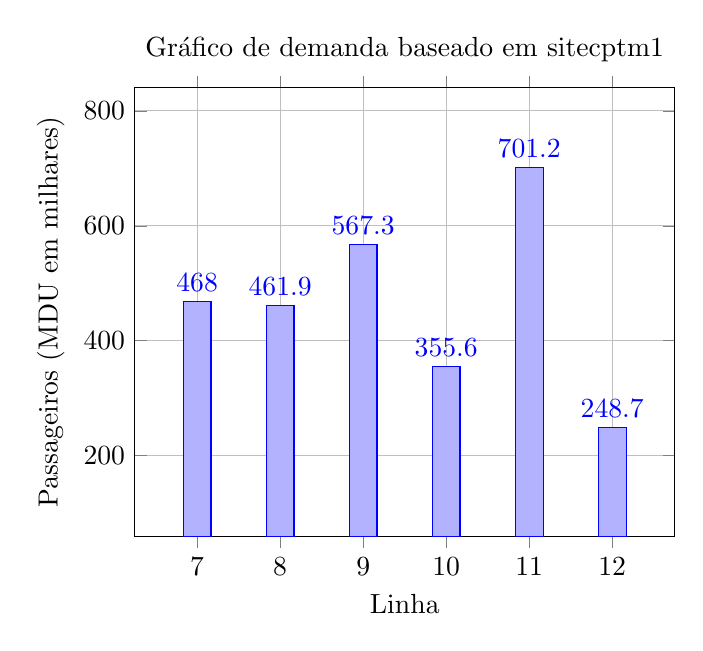
\begin{tikzpicture}
		\begin{axis}[
		title=Gráfico de demanda baseado em \citeonline{sitecptm1},
		grid=both,
		ymin=150,
		ymax=750,
		ybar,
		symbolic x coords={7,8,9,10,11,12},
		nodes near coords, nodes near coords align={vertical},
		xlabel=Linha,
		ylabel=Passageiros (MDU em milhares),
		enlargelimits=0.15,
		]
		\addplot+[ybar] coordinates
		{(7,468.000)
		(8,461.900)
		(9,567.300)
		(10,355.600)
		(11,701.200)
		(12,248.700)};
		\end{axis}
		\end{tikzpicture}
	\end{center}

	Das 92 estações totais do sistema, 56 delas se inserem no contexto deste trabalho (60,9\% de toda a malha), onde apenas 11 serão abordadas de forma mais ou menos direta (12\% de toda a malha de todas as estações, 19,6\% inseridas no contexto), dependendo do assunto a ser relacionado no próximo capítulo, outrossim, a tabela a seguir busca sumarizar e clarificar a abrangência em relação à malha do Trem Metropolitano.
	
	\begin{center}
		\begin{longtable}{|l|l|l|l|}
			\caption{Tabela comparativa do alcance deste trabalho, elaborada com base em \cite{sitecptm2}}\\
			\hline
			\textbf{Comparação} & \textbf{Estações (A)} & \textbf{Estações (B)} & \textbf{Percentagem} \\
			\hline
			\endfirsthead
			\multicolumn{4}{c}%
			{\tablename\ \thetable\ -- \textit{Continuado da página anterior}} \\
			\hline
			\textbf{Comparação} & \textbf{Estações} & \textbf{Estações} & \textbf{Percentagem} \\
			\hline
			\endhead
			\hline \multicolumn{4}{r}{\textit{Continua na próxima página}} \\
			\endfoot
			\hline
			\endlastfoot
			Contexto (A) $\times$ Alcance (B) & 56 & 11 & 19,6\% \\
			Rede (A) $\times$ Contexto (B) & 92 & 56 & 60,9\% \\
			Rede (A) $\times$ Alcance (B) & 92 & 11 & 12,0\% \\
		\end{longtable}
	\end{center}
	
	Para os dados de demanda, apontados em subseções homônimas nos próximos capítulos, todos foram baseados em dados cedidos pela Mídia CPTM, responsável pela publicidade nos trens e estações, sendo as referências: \citeonline{tabcptm201501}, \citeonline{tabcptm201502}, \citeonline{tabcptm201503}, \citeonline{tabcptm201506}, \citeonline{tabcptm201510}, \citeonline{tabcptm201401}, \citeonline{tabcptm201402}, \citeonline{tabcptm201403}, \citeonline{tabcptm201404}, \citeonline{tabcptm201405}, \citeonline{tabcptm201407}, \citeonline{tabcptm201409}, \citeonline{tabcptm201410}, \citeonline{tabcptm201411}, \citeonline{tabcptm201412}, \citeonline{tabcptm201301}, \citeonline{tabcptm201302}, \citeonline{tabcptm201303}, \citeonline{tabcptm201304}, \citeonline{tabcptm201305}, \citeonline{tabcptm201307}, \citeonline{tabcptm201308}, \citeonline{tabcptm201309}, \citeonline{tabcptm201310}, \citeonline{tabcptm201311}, \citeonline{tabcptm201312}, \citeonline{tabcptm201204}, \citeonline{tabcptm201205}, \citeonline{tabcptm201207}, \citeonline{tabcptm201208}, \citeonline{tabcptm201209}, \citeonline{tabcptm201210}, \citeonline{tabcptm201211}, \citeonline{tabcptm201108}, \citeonline{tabcptm201109}, \citeonline{tabcptm201110}, \citeonline{tabcptm201111}, \citeonline{tabcptm201112}. A utilização de ``Mídia CPTM'' a partir daqui implica nestas referências, correspondentes às tabelas de movimentação disponíveis e obtidas por mim entre 2011 e 2015.

%
%==============================================================================================	
%
	\chapter{A rede como fio-condutor}
	
	Este capítulo explora as relações sócio-territoriais a partir de casos definidos com base em uma linha e um conjunto de estações, estabelecendo um diálogo que tanto permite limitar a área estudada, como também reforça o papel coesivo do Trem Metropolitano, não no sentido de harmonizar o território ou suprimir seus conflitos, embora tal possibilidade não possa ser descartada, mas coesivo no sentido infraestrutural, como elemento durável, referencial e articulador\footnote{``(\dots) os tempos dos retornos dos investimentos feitos na ferrovia são normalmente diferentes daqueles de outros investimentos e, principalmente, as suas
	características influem na localização das demais atividades humanas, modificam a paisagem de forma indelével, mesmo após seu abandono.''\apud[pág. ~13]{Ferreira}{Merlin}}.
	
	Sendo a malha da CPTM um elemento estruturante e gerida pelo governo estadual de São Paulo, apesar do enfraquecimento do papel do estado no planejamento do território, vale destacar que a mesma esfera de poder conta com uma estatal dedicada ao planejamento territorial da \gls{rmsp} e outras regiões metropolitanas, vide \citeonline[p. 224]{Stefani}, ``Cabe à \gls{emplasa} a execução de assessoramento ao Governo do Estado de São Paulo para questões metropolitanas. Nesse sentido, elabora projetos de uso e ocupação do solo, de urbanização e revitalização urbana, planos regionais e sub regionais, estudos sócio-econômicos e políticos. Presta ainda, assessoria técnica aos municípios do complexo metropolitano expandido: Grande São Paulo, Baixada Santista e Campinas, além das concentrações urbanas do Vale do Paraíba, Sorocaba e outras áreas de seu entorno.''
	
	%\begin{citacao}
	%	Instaura-se então o que Harvey chamou de “reversão competitiva”, em que não mais o capital busca vantagens locacionais, mas as localidades	é que competem entre si, oferecendo vantagens locacionais para atrair os capitais \apud{Acselrad}{Harvey1995}. A chamada “governança urbana” institui uma multiplicidade de pólos de iniciativa e decisão, envolvendo atores não-governamentais, semipúblicos e privados. Uma tal “flexibilização” institucional veio favorecer fortemente os segmentos empresariais, através dos mecanismos de negociação das normas urbanísticas, liberação do controle do uso do solo, renúncia fiscal e subsídio ao investimento privado, mediante a oferta de infra-estrutura, terrenos, formação de mão-de-obra etc.\apud{Acselrad}{Silva2001}
	%\end{citacao}

%
%==============================================================================================	
%

	\section{Linha 8-Diamante: fragmentação}
	
	Aqui me restringirei às estações compreendidas nas cidades de Osasco, Carapicuíba e Barueri, sobretudo no tocante ao acesso à região de Alphaville, embora seja válido e importante destacar o peso econômico de Osasco e a existência de um polo atrator de viagens, baseado, sobretudo, no setor comerciário.
	
	\begin{figure}[h]
		\caption{Mapa da Linha 8 exibido dentro de um trem (2015)}
		\includegraphics[keepaspectratio,width=\textwidth]{fotos/DSCN8143.JPG}
	\end{figure}
	
	% feito - FALTAM CITAÇÕES A PARTIR DAQUI
	% podem ser obtidas em https://medium.com/trens-metropolitanos/os-tropeços-na-reconstrução-da-estação-antônio-joão-30ecbcddb802
	%
	A Linha 8 permite uma oportuna exploração da fragmentação urbana provocada por Alphaville, não só por se correr paralela, ainda que não adjacente, a parcelas consideráveis do empreendimento, que podem se fazer notar entre o trecho compreendido pelas estações Carapicuíba e Barueri, sendo também importante o papel da Estação General Miguel Costa, como veremos a seguir. Basicamente, a análise se apoiará nas estações Antônio João, em Barueri e General Miguel Costa, na divisa de Osasco e Carapicuíba, terminando com comentários de maior brevidade em relação à Estação Barueri, localizada no município homônimo.
	
	\subsection{Estação Antônio João}
	% acho que terminei o que faltava - AJO
	%
	Visitar a Estação Antônio João permite observar o processo de anacronismo pelo qual ela tem passado, relacionado por transformações não só nos serviços da \gls{cptm}, como também na região em que está inserida (Aldeia de Barueri). Antônio João, cada vez mais, mostra ser uma estação que estagnou, cujas formas e ambiência aludem a uma realidade que há muito deixou de existir.
	
	\begin{figure}[h]
		\caption{Estação Antônio João vista a partir do viaduto (2015)}
		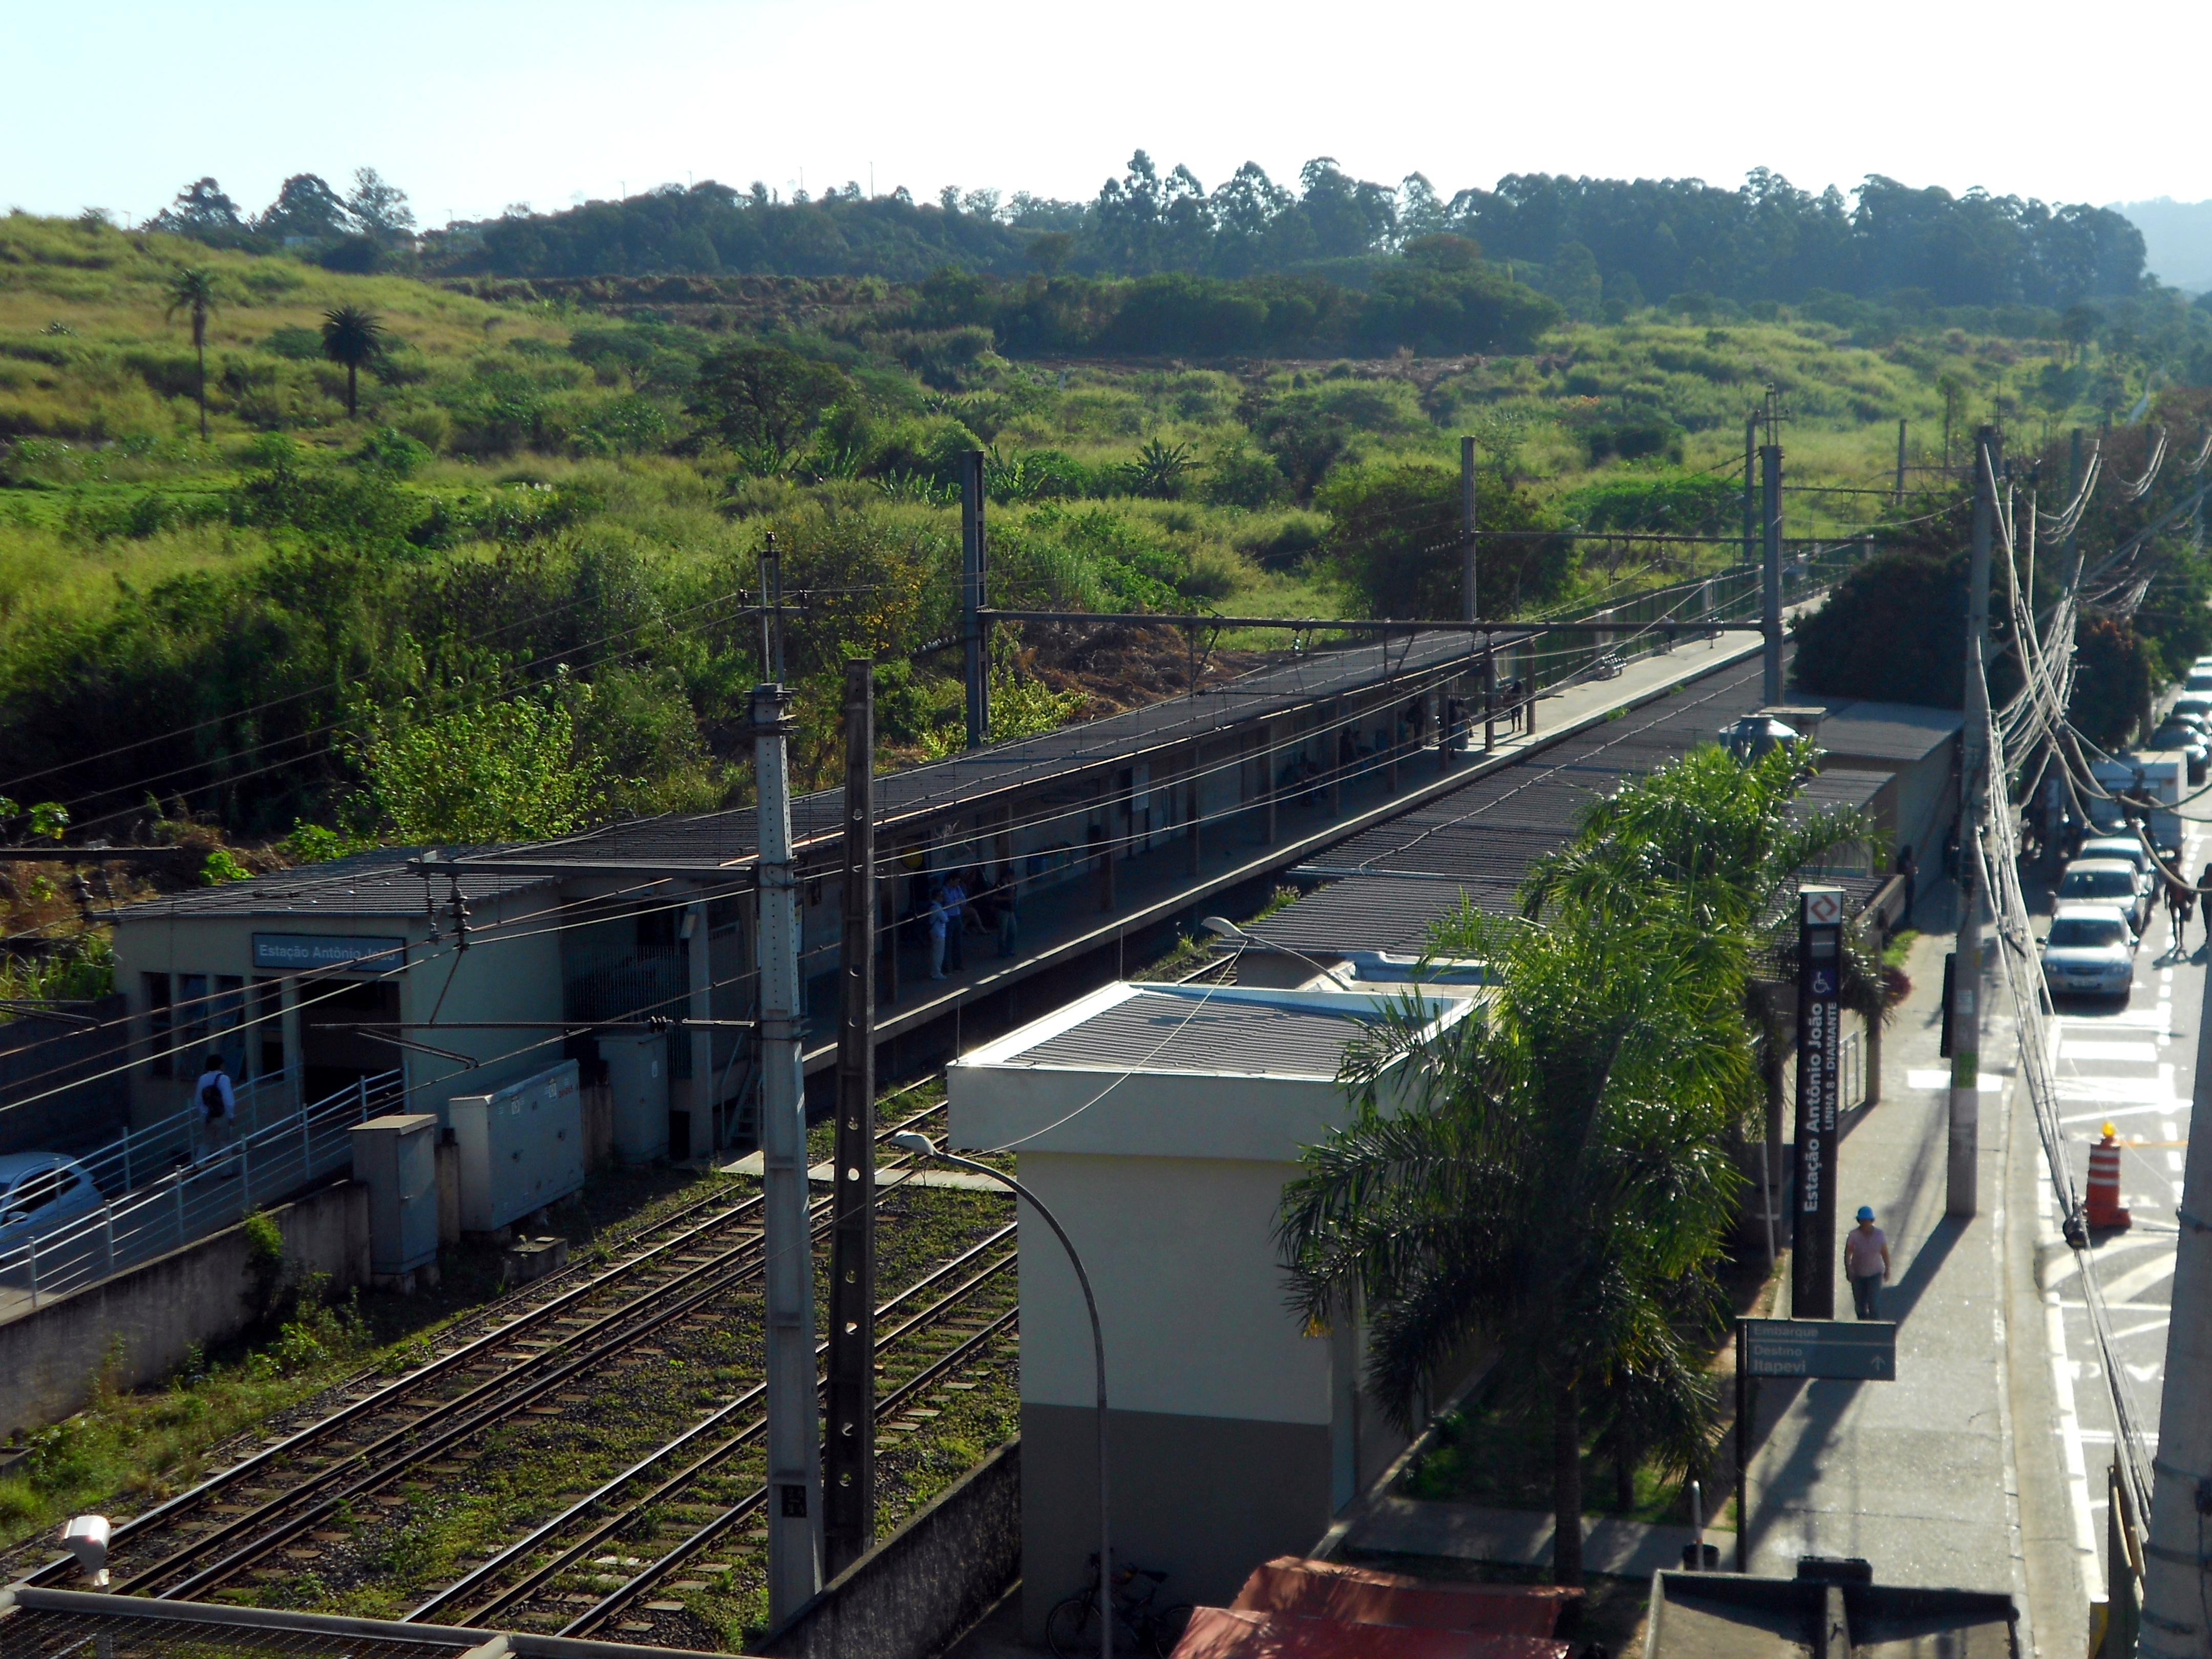
\includegraphics[keepaspectratio,width=\textwidth]{fotos/DSCN8163.JPG}
	\end{figure}
	
	Não fosse pela chegada da CSU em 2009, cujas instalações na época foram alardeadas como sendo as do maior \textit{call center} da América Latina\cite{investesp}, talvez Antônio João continuasse exibindo um certo ar bucólico, apesar disso, com a chegada do viaduto, cerca de dez anos atrás, aqueles que nele passaram transitar ganharam não só uma forma de transposição, mas também uma visão privilegiada de edifícios corporativos na região empresarial de Alphaville, ou seja, já havia, pelo menos, um potencial para que Antônio João atuasse como uma espécie de \textit{hub}\footnote{Nó concentrador, com infraestrutura capaz de abrigar múltiplas linhas e modos de transporte.}, com destaque para a intermodalidade (integração entre diferentes modos de transporte). O edifício da CSU pode ser visto da estação, causando um misto de impacto e contraste, fazendo a estação parecer simplesmente fora do lugar, perdida em nossa época, o que se soma ao aspecto da via permanente\footnote{Brita, trilhos, dormentes e outros elementos que compõem a via férrea como um todo.} contribui, transmitindo desleixo por parte do poder público estadual.
	
	\begin{figure}[h]
		\caption{A região de Alphaville Barueri observada a partir do viaduto conectado à Estação Antônio João (2015)}
		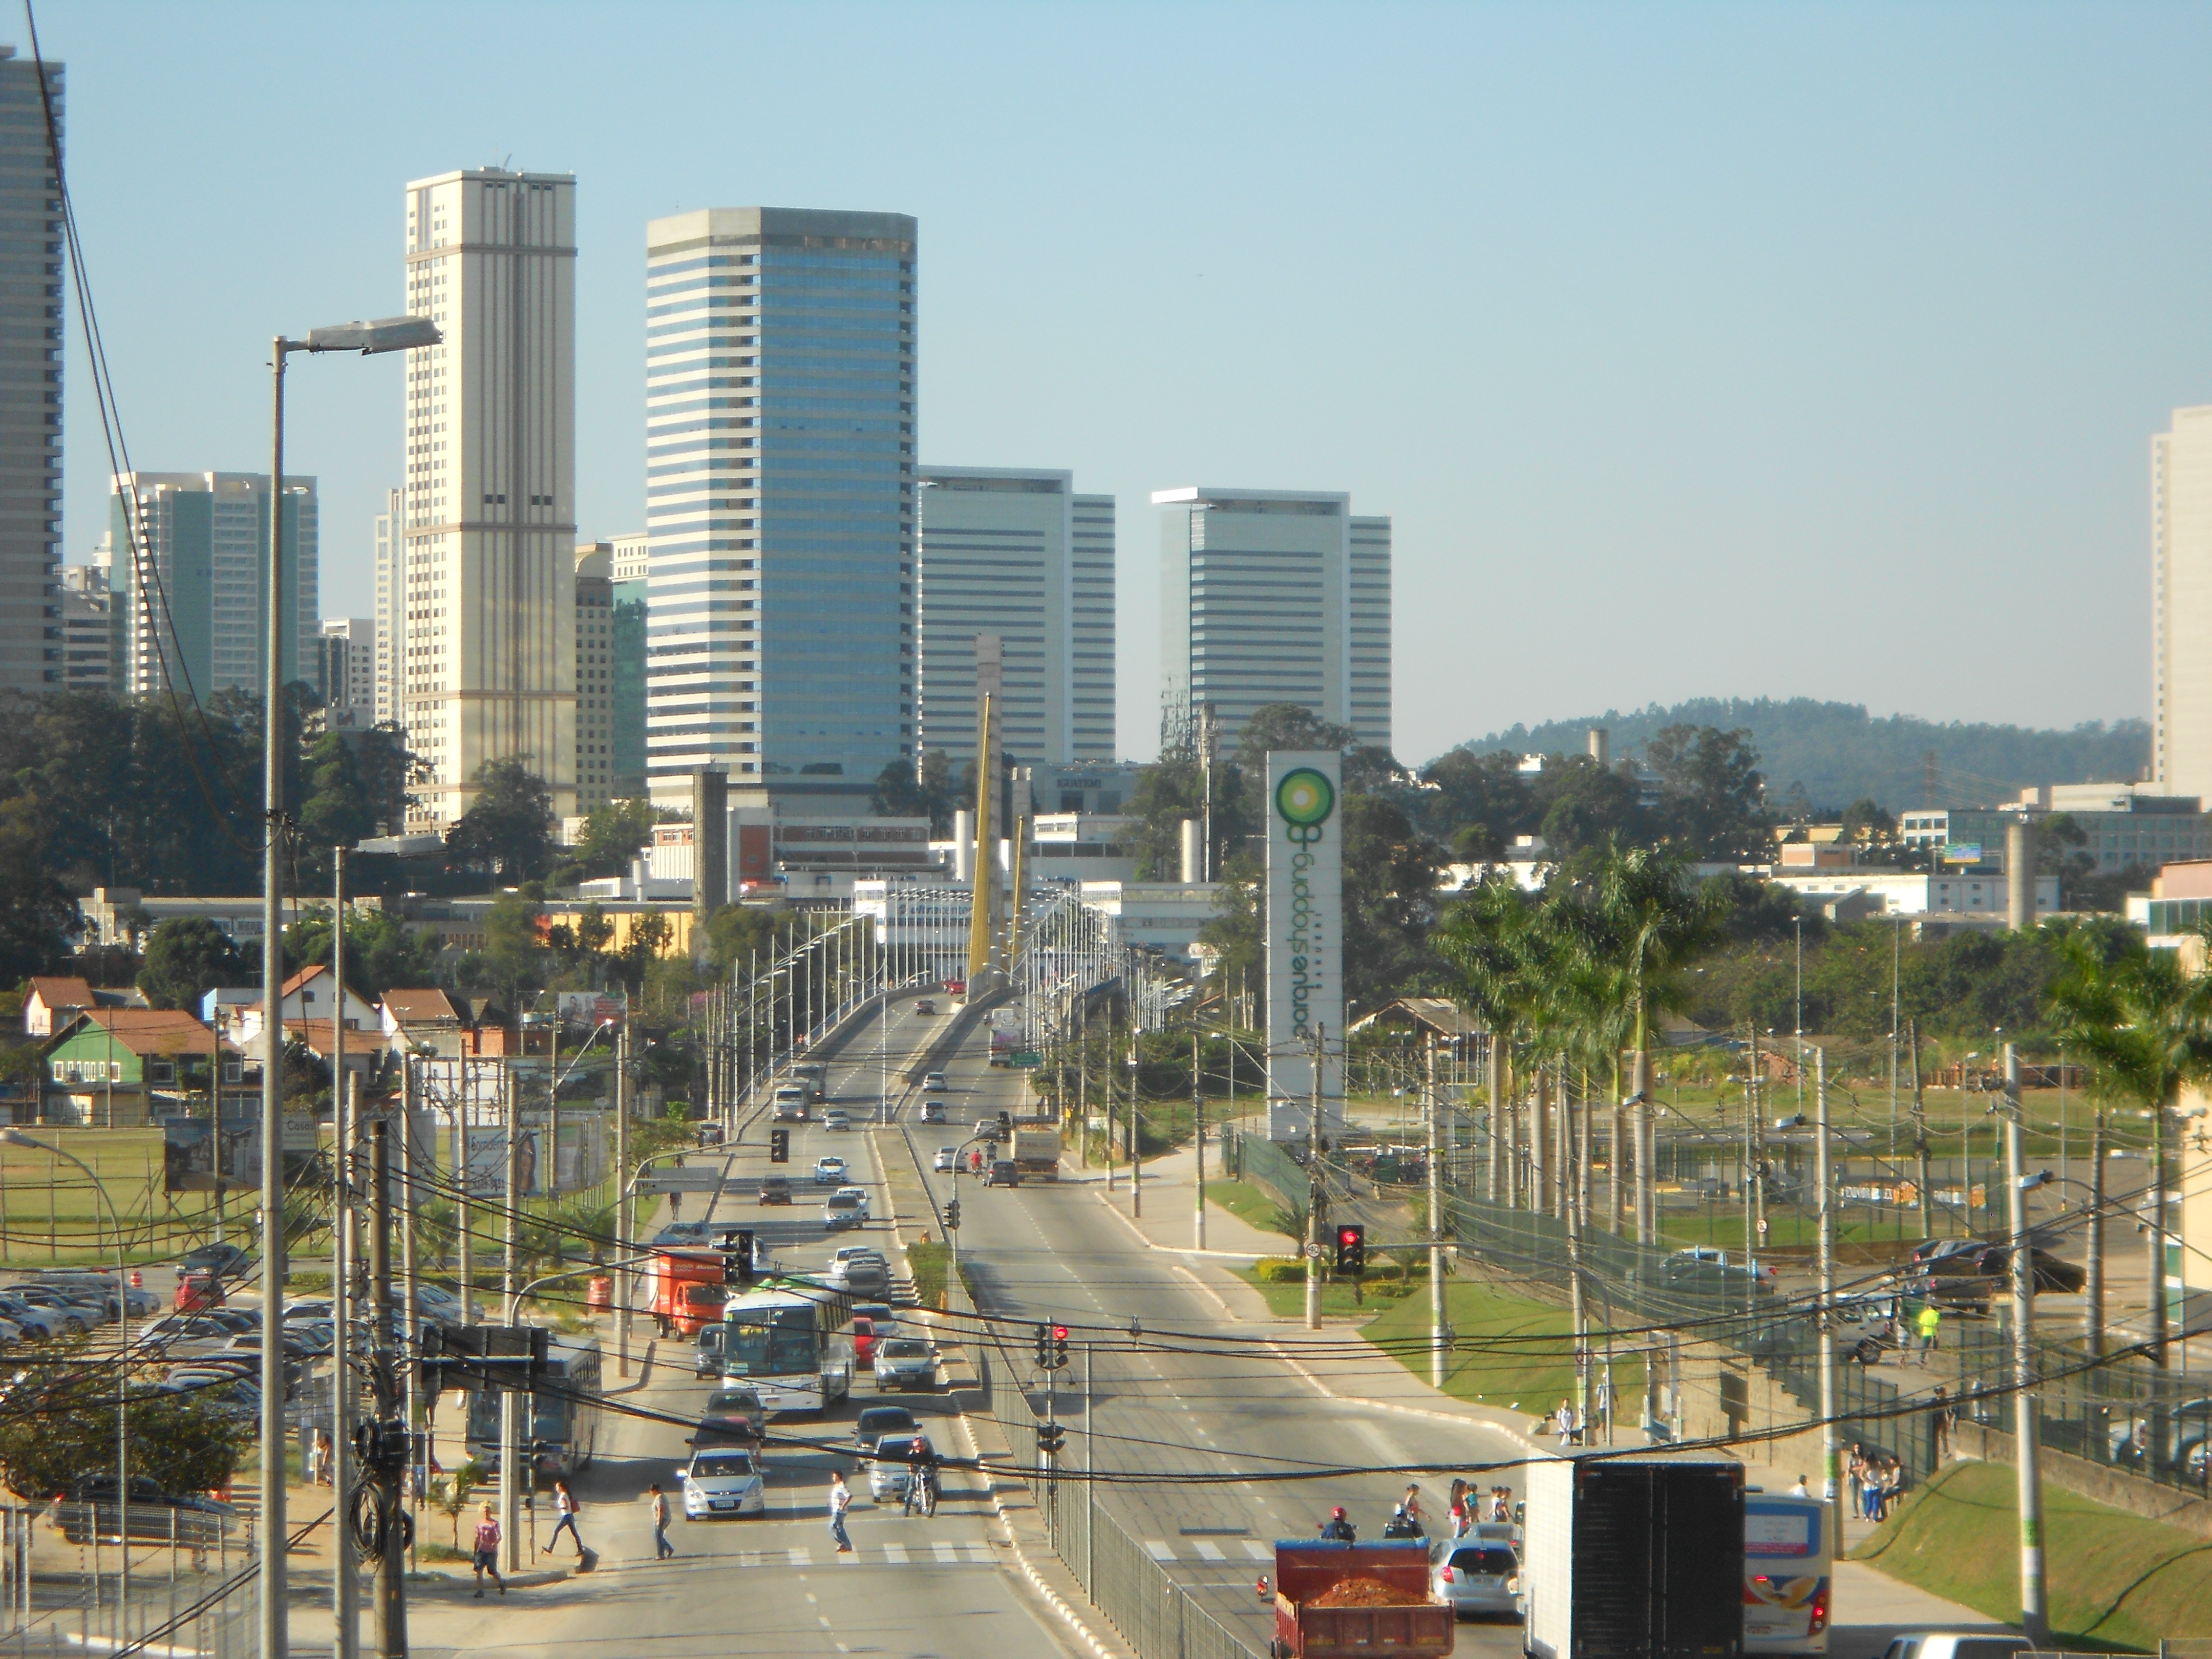
\includegraphics[keepaspectratio,width=\textwidth]{fotos/DSCN8173.JPG}
	\end{figure}
	
	O acesso ao viaduto é feito por uma escada metálica, que não tem uma aparência das mais simpáticas. A \gls{cptm} disponibiliza uma passagem de nível\footnote{Passagem pela qual podem passar, em nível, ou seja, na mesma altura dos trilhos, pedestres e/ou veículos.} na estação, intencionada principalmente para utilização por deficientes físicos que permite passar de um lado para o outro, o que remedia a situação de forma bastante precária.
	
	Vale notar que apenas em 2006 a Prefeitura de Barueri concluiu a pavimentação nas imediações do acesso localizado na plataforma sentido Júlio Prestes da estação: ``Na Aldeia de Barueri, o bairro está recebendo os últimos serviços de conclusão das vias do novo Centro Empresarial, em frente à estação Antônio João da CPTM. A avenida General de Divisão Pedro Rodrigues da Silva foi ampliada e ganhou uma rotatória''\cite{barueri}.

	Não significa, porém, que tenha estabelecido uma ligação rodoviária margeando os trilhos. Até agosto de 2015, tapumes e cones deixavam claro que a lama apenas cedera seu lugar a uma avenida incompleta.
	
	% feito - EXISTE POSSIBILIDADE DE RECLAMAR DO MAU PEDESTRIANISMO USANDO FALCONE
	%
	Na mesma rua do viaduto (General de Divisão Pedro Rodrigues da Silva), existe um semáforo que permite acesso ao Parque Shopping, inaugurado em novembro de 2011 e contando com \gls{abl} de 34,4 mil m$^2$ \cite{valoreconomico}, bem como ao ponto de ônibus situado próximo do mesmo centro comercial. Notoriamente essa região continua não sendo projetada com o pedestre em mente, que perde um bom tempo para atravessar de um lado ao outro se agir corretamente, esperando o semáforo da mesma rua do viaduto (General de Divisão Pedro Rodrigues da Silva). É o semáforo em conjunto com uma faixa de pedestres que permite acesso ao Parque Shopping e ao ponto de ônibus situado próximo do mesmo centro comercial. Seu tempo de abertura e fechamento claramente prioriza o automóvel. Finalmente, além do semáforo com temporização que prioriza o transporte individual motorizado em detrimento ao pedestre, não há faixa exclusiva de ônibus ou ciclovia, o que reforça a visão do poder público local, exibida já nos pontos de ônibus existentes, pequenos para a demanda gerada pelo polo de comércio e serviços que atualmente se encontra instalado. 	Apesar de não contar com uma infraestrutura de integração física dedicada, a estação é atendida por três linhas de ônibus, conforme levantamento junto ao poder público local e à empresa responsável pela operação. Das quatro linhas de ônibus, duas atendem o empreendimento: T244 e T245VP1, esta última criada apenas em setembro de 2015\cite{visao}.

	% aplicando workaround http://tex.stackexchange.com/questions/276699/the-longtable-environment-pushes-content-below-it-into-the-bottom-margin-of-a-pa#comment668108_276699
	\begin{minipage}[t]{0.5 \linewidth}
	\begin{center}
		\begin{longtable}{|l|l|p{4.5cm}|p{4.5cm}|}
			\caption{Tabela com as linhas de ônibus na Estação Antônio João}\\
			\hline
			\textbf{Linha} & \textbf{Tipo} & \textbf{Viagem de Ida} & \textbf{Viagem de Volta} \\
			\hline
			\endfirsthead
			\multicolumn{4}{c}%
			{\tablename\ \thetable\ -- \textit{Continuado da página anterior}} \\
			\hline
			\textbf{Linha} & \textbf{Tipo} & \textbf{Viagem de Ida} & \textbf{Viagem de Volta} \\
			\hline
			\endhead
			\hline \multicolumn{4}{r}{\textit{Continua na próxima página}} \\
			\endfoot
			\hline
			\endlastfoot
			A111 & BBTT & Estação Antônio João & Vila Márcia  \\
			A112 & BBTT & Estação Antônio João & Barueri (Centro) \\
			T244 & BBTT & Vale do Sol  & Tamboré \\
			T245VP1 & BBTT & Estação Antônio João & 18 do Forte \\
			\hline
		\end{longtable}
	\end{center}
	\end{minipage}

	% citando Falcone aqui e matando a pendência
	A postura negligente com relação ao pedestre também foi destacada por \citeonline{Falcone}: ``Embaixo dos viadutos e nas rotatórias têm sido feitos praças e jardins de caráter meramente cenográfico, pois se encontram em meio a vias de tráfego rápido e dificilmente podem ser usufruídas pelo pedestre. O tratamento paisagístico também é cenográfico, com lagos artificiais e cascatas, pontes japonesas e cascalho branco. A intenção é o embelezamento das principais vias de acesso à cidade, causando boa impressão ao visitante, ou ao empresário que deseja instalar-se no município. Perto desses acessos, os poucos espaços livres públicos utilizados para lazer da população, como a pista de	caminhada ao lado do Rio Tietê, encontram-se em péssimo estado de conservação''.
	
	\subsection{Estação General Miguel Costa}
	Localiza-se na divisa dos municípios de Osasco e Carapicuíba, a Estação General Miguel Costa, figurando como um importante \textit{hub}, que por meio da intermodalidade\footnote{Intermodalidade: ``Uma das formas de reorganizar os sistemas de transporte público, objetivando a racionalização, a redução de custos e o aumento da mobilidade''\apud{Nabais}{ANTP} ou ``Um conjunto de medidas de natureza físico-operacional, tarifária e institucional destinadas a articular e racionalizar os serviços de		transporte público''\apud{Nabais}{Cadaval}.}com os ônibus, permite acesso a Alphaville, sendo também notável por ter sido escolhida para receber um terminal de ônibus integrado ao futuro Corredor Metropolitano Itapevi - São Paulo da \gls{emtu}. A opção pela rodovia, intrínseca ao desenvolvimento de Alphaville, torna oportuna a menção por concentrar dezenas de linhas de ônibus. Sobre a opção pela rodovia e a ausência de articulação direta entre o empreendimento e o transporte sobre trilhos, \citeonline{Falcone} destaca que:
	\begin{citacao}
		A implantação de Alphaville foi favorecida pela abertura da Rodovia Castello Branco, que possibilitou a ligação do empreendimento ao vetor sudoeste da capital.
		
		Ainda hoje, não há uma ligação com o trem metropolitano da CPTM ou um sistema de transporte público eficaz capaz de conectar Alphaville à capital, e mesmo aos municípios do entorno. Pode-se dizer que o elemento estruturador de Alphaville/Tamboré é o viário. Um conjunto de vias mal hierarquizadas conecta os diversos setores do empreendimento: industrial, empresarial, comercial e residencial.
		\cite[pág. 125]{Falcone}
	\end{citacao}
	
	% feito - COLOCAR FOTO DO INTERMUNICIPAL COM PASSAGEIROS NO PONTO, DE FRENTE
	\begin{figure}[tp]
		\caption{Ônibus intermunicipal no Alphaville Empresarial (2015)}
		\includegraphics[keepaspectratio,width=\textwidth]{fotos/DSCN8531.JPG}
	\end{figure}
	
	Conforme \citeonline[pág. 31]{Acselrad}:``A fragmentação por baixo, sugere-nos \citeonline{Jaglin}, decorre de uma concepção comunitarista de solidariedade, que promove um parcelamento gestionário dos bairros pobres, uma descontinuidade física das redes de ilhas selecionadas de atendimento, gerando competição entre as comunidades e no interior das mesmas por recursos escassos. A fragmentação pelo alto, por sua vez, reúne todas as formas de dessolidarização entre áreas ricas e áreas pobres, de renúncia ao compartilhamento fiscal, tarifário e de redes de infra-estrutura, além das práticas de auto-segregação espacial, via condomínios fechados, gradeamento, segurança privada etc''. A auto-segregação espacial e a renúncia à infraestrutura ferroviária de transporte metropolitano é um traço indissociável do que Alphaville representa, estabelecendo um diálogo direto com a Linha 8 da \gls{cptm}, não pela articulação direta do empreendimento, como apontei acima, mas pela fragmentação que ele provoca ao não adotá-la, procurando constituir um espaço apartado do restante do município de Barueri\footnote{Alphaville também avança sobre o território de Santana de Parnaíba, contudo, não se trata de um município atendido pelo Trem Metropolitano.}. \citeonline[pág. 31]{Acselrad} ainda destaca que os empreendimentos possuem como características: utilização de muros ou grades (muros são observados em todos os residenciais de Alphaville), acesso restrito e controlado, aparato interno de segurança e vigilância, residentes conectados entre si por um código de conduta comum.

	Por meio de levantamento de informações públicas fornecidas pela \gls{emtu} e empresas responsáveis pelas linhas de ônibus em Osasco e Carapicuíba, identifiquei que hoje há um total de 30 linhas junto à Estação General Miguel Costa, sendo que nenhuma das 21 linhas intermunicipais faz terminal na estação, enquanto 7 das 9 linhas municipais fazem terminal na estação. Para todos os casos a situação é inadequada devido à falta de infraestrutura de integração e abrigo dos ônibus e passageiros. É também flagrante que as linhas não respeitam o horário de operação do Trem Metropolitano. O serviço de metropolitanos da \gls{cptm} opera diariamente das 4h à 0h00, sendo que aos sábados o funcionamento cessa à 1h00\cite{sitecptm3}.
	
	\begin{center}
		\begin{longtable}{|l|l|p{4.5cm}|p{4.5cm}|}
			\caption{Tabela com as linhas de ônibus na Estação General Miguel Costa}\\
			\hline
			\textbf{Linha} & \textbf{Tipo} & \textbf{Viagem de Ida} & \textbf{Viagem de Volta} \\
			\hline
			\endfirsthead
			\multicolumn{4}{c}%
			{\tablename\ \thetable\ -- \textit{Continuado da página anterior}} \\
			\hline
			\textbf{Linha} & \textbf{Tipo} & \textbf{Viagem de Ida} & \textbf{Viagem de Volta} \\
			\hline
			\endhead
			\hline \multicolumn{4}{r}{\textit{Continua na próxima página}} \\
			\endfoot
			\hline
			\endlastfoot
			130 & EMTU & SAO PAULO (LAPA) & JANDIRA (JARDIM NOSSA SENHORA DE FATIMA) \\
			133 & EMTU & OSASCO (CENTRO) & ITAPEVI (COHAB/JARDIM PAULISTA) \\
			133BI1 & EMTU & OSASCO (CENTRO) & ITAPEVI (VILA GIOIA) \\
			223 & EMTU & OSASCO (VILA YARA) & CARAPICUIBA (COHAB V) \\
			224 & EMTU & SAO PAULO (LAPA) & CARAPICUIBA (COHAB V) \\
			225 & EMTU & SAO PAULO (PINHEIROS) & CARAPICUIBA (COHAB V) \\
			345 & EMTU & SAO PAULO (LAPA) & BARUERI (VALE DO SOL) \\
			350 & EMTU & SAO PAULO (TERMINAL RODOVIARIO BARRA FUNDA) & ITAPEVI (COHAB) \\
			350BI1 & EMTU & SAO PAULO (TERMINAL RODOVIARIO BARRA FUNDA) & ITAPEVI (VILA GIOIA) \\
			390 & EMTU & BARUERI (ALPHAVILLE 3 / BRADESCO) & OSASCO (JARDIM VELOSO) \\
			420 & EMTU & OSASCO (CENTRO) & COTIA (PARQUE SANTA RITA) \\
			428 & EMTU & SAO PAULO (METRO BUTANTA) & BARUERI (JARDIM DO LIBANO) \\
			448 & EMTU & SANTANA DE PARNAIBA (RESIDENCIAL TAMBORE III) & CARAPICUIBA (PARQUE JANDAIA) \\
			449 & EMTU & SANTANA DE PARNAIBA (ALPHAVILLE 10) & CARAPICUIBA (PARQUE JANDAIA) \\
			450 & EMTU & BARUERI (ALPHAVILLE 2) & CARAPICUIBA (JARDIM NOVO HORIZONTE) \\
			458 & EMTU & SAO PAULO (TERMINAL RODOVIARIO BARRA FUNDA) & CARAPICUIBA (COHAB I) \\
			496 & EMTU & SAO PAULO (JARDIM JOAO XXIII) & BARUERI (ALPHAVILLE 3 / BRADESCO) \\
			516 & EMTU & SAO PAULO (METRO BUTANTA) & JANDIRA (JARDIM NOSSA SENHORA DE FATIMA) \\
			539 & EMTU & OSASCO (CENTRO) & ITAPEVI (COHAB/JARDIM PAULISTA) \\
			557 & EMTU & SAO PAULO (LAPA) & JANDIRA (JARDIM NOSSA SENHORA DE FATIMA) \\
			579 & EMTU & BARUERI (ALPHAVILLE 3 / BRADESCO) & OSASCO (VILA YOLANDA) \\
			581 & EMTU & COTIA (KM 24 - RODOVIA RAPOSO TAVARES) & CARAPICUIBA (ESTACAO GENERAL MIGUEL COSTA - KM 21) \\
			013 & DEL REY & ESTAÇÃO KM 21 & JD. TONATO \\
			022 & DEL REY & ESTAÇÃO KM 21 & PARQUE JANDAIA \\
			023 & DEL REY & ESTAÇÃO KM 21 & JARDIM ANGÉLICA \\
			024 & DEL REY & ESTAÇÃO CENTRO & COHAB V \\
			106 & ETT & VILA GÁLIA & OLARIA \\
			108 & ETT & ESTAÇÃO KM 21 & VILA HELENA \\
			109 & ETT & ESTAÇÃO KM 21 & PQ. SANTA TEREZA \\
			111 & ETT & ESTAÇÃO KM 21 & NOVO HORIZONTE \\
			005 & V. OSASCO & EST. CPTM GAL. MIGUEL COSTA (KM 21) & VILA YARA \\
		\end{longtable}
	\end{center}
	
	Mesmo que o passageiro seja beneficiado pelo horário ampliado aos sábados, por exemplo, não encontrará 29 das 30 linhas de ônibus nas imediações, já que apenas a linha 225 tem horários com maior grau de compatibilidade com a \gls{cptm}, adicionalmente, 6 das 31 linhas fazem menção direta a Alphaville: 390, 448, 449, 450, 496 e 579, reunidas na lista a seguir.
	
	\begin{center}
		\begin{longtable}{|l|l|p{5cm}|p{5cm}|}
			\caption{Tabela com as linhas de ônibus na Estação General Miguel Costa que atendem Alphaville}\\
			\hline
			\textbf{Linha} & \textbf{Tipo} & \textbf{Viagem de Ida} & \textbf{Viagem de Volta} \\
			\hline
			\endfirsthead
			\multicolumn{4}{c}%
			{\tablename\ \thetable\ -- \textit{Continuado da página anterior}} \\
			\hline
			\textbf{Linha} & \textbf{Tipo} & \textbf{Viagem de Ida} & \textbf{Viagem de Volta} \\
			\hline
			\endhead
			\hline \multicolumn{4}{r}{\textit{Continua na próxima página}} \\
			\endfoot
			\hline
			\endlastfoot
			390 & EMTU & BARUERI (ALPHAVILLE 3 / BRADESCO) & OSASCO (JARDIM VELOSO) \\
			448 & EMTU & SANTANA DE PARNAIBA (RESIDENCIAL TAMBORE III) & CARAPICUIBA (PARQUE JANDAIA) \\
			449 & EMTU & SANTANA DE PARNAIBA (ALPHAVILLE 10) & CARAPICUIBA (PARQUE JANDAIA) \\
			450 & EMTU & BARUERI (ALPHAVILLE 2) & CARAPICUIBA (JARDIM NOVO HORIZONTE) \\
			496 & EMTU & SAO PAULO (JARDIM JOAO XXIII) & BARUERI (ALPHAVILLE 3 / BRADESCO) \\
			579 & EMTU & BARUERI (ALPHAVILLE 3 / BRADESCO) & OSASCO (VILA YOLANDA) \\
		\end{longtable}
	\end{center}
	
	Como um importante polo comercial, empresarial e industrial, Alphaville demanda muita mão de obra, sendo que a maioria dos trabalhadores não mora nos residenciais fechados, conclusão talvez óbvia, mas que fica reforçada pelo periódico britânico The Guardian, segundo o qual Alphaville é um dos dez maiores muros do planeta\cite{muro}.
	
	\begin{citacao}
		Com um contingente de 154.606 trabalhadores, Alphaville tem um número três vezes menor de moradores, 43.521. Os índices econômicos da população fixa são superlativos: $76,3$\% dos domicílios possuem renda mensal acima de 11.000 reais; em São Paulo são $16,7$\%. A média é de 16.724 reais -- contra 3.427 reais da capital, segundo dados da Cognatis Geomarketing.
		\cite{poloadm}
	\end{citacao}
	
	Com sua atual configuração, que pouco sofreu alterações ao longo de décadas, a Estação General Miguel Costa não configura qualquer tipo de ligação eficaz entre o sistema metroferroviário e Alphaville, se limitando a um nó de conexão entre os metropolitanos da \gls{cptm} e os ônibus intermunicipais da \gls{emtu}. Sem infraestrutura adequada, tal quadro se soma com o da ainda mais frágil Estação Antônio João.
	
	\subsection{Estação Barueri}
	
	Em comparação com as outras duas situações, aqui há um quadro de evolução, principalmente nos termos de uma intermodalidade facilitada, pois a estação principal da cidade, e que leva o nome do município, é vizinha a um terminal de ônibus coberto (batizado de Terminal Rodoferroviário Gualberto Tolaine).
	
	\begin{figure}[h]
		\caption{Terminal de ônibus fronteiriço à Estação Barueri (2016)}
		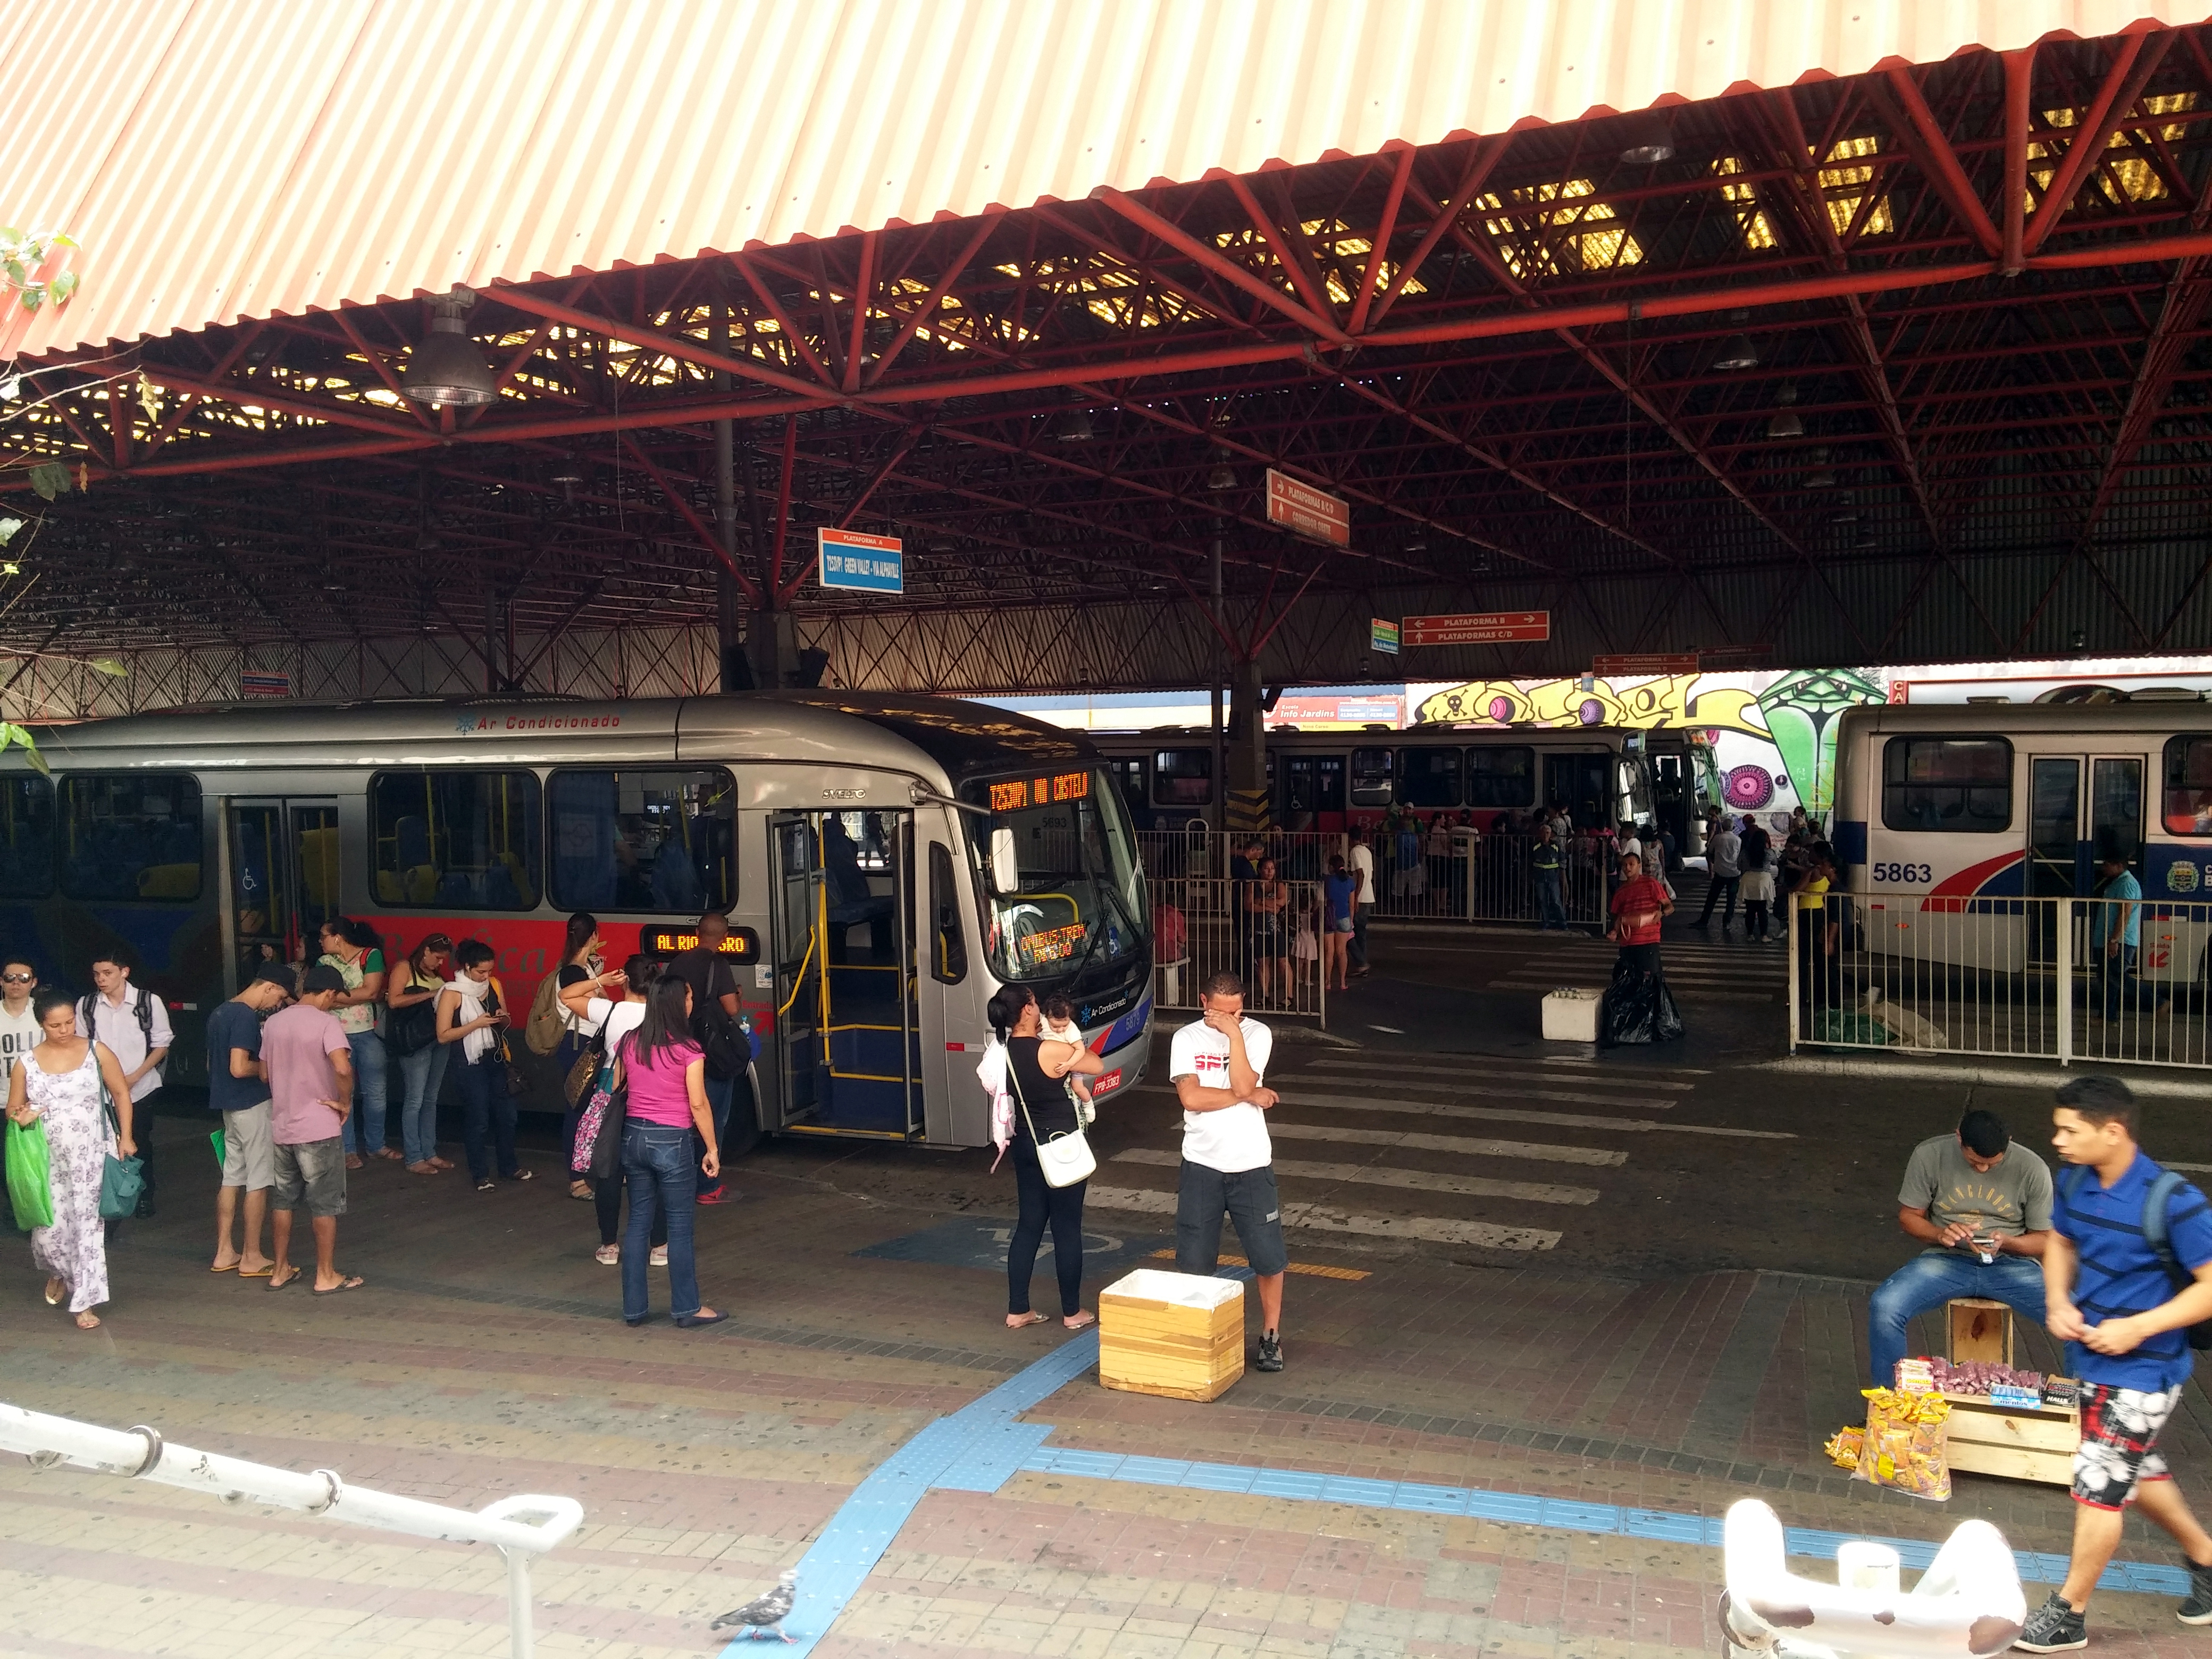
\includegraphics[keepaspectratio,width=\textwidth]{fotos/20160413_152547.jpg}
	\end{figure}

	Em mapeamento das linhas realizado por mim, conforme levantamento feito em visita ao local e também com base nas informações disponibilizadas pelo poder público e empresa responsável pela operação ({\glsdesc*{bbtt}}), foram identificadas 23 linhas de ônibus utilizando a infraestrutura do terminal.	
	
	\begin{center}
		\begin{longtable}{|l|l|p{4.5cm}|p{4.5cm}|}
			\caption{Tabela com as linhas de ônibus na Estação Barueri}\\
			\hline
			\textbf{Linha} & \textbf{Tipo} & \textbf{Viagem de Ida} & \textbf{Viagem de Volta} \\
			\hline
			\endfirsthead
			\multicolumn{4}{c}%
			{\tablename\ \thetable\ -- \textit{Continuado da página anterior}} \\
			\hline
			\textbf{Linha} & \textbf{Tipo} & \textbf{Viagem de Ida} & \textbf{Viagem de Volta} \\
			\hline
			\endhead
			\hline \multicolumn{4}{r}{\textit{Continua na próxima página}} \\
			\endfoot
			\hline
			\endlastfoot
			A111 & BBTT & Estação Antônio João & Vila Márcia  \\
			A112 & BBTT & Estação Antônio João & Barueri (Centro) \\
			A163 & BBTT & Jd. Maria Cristina & Chácara Marcos via Jd. São Silvestre \\
			A164 & BBTT & Barueri (Centro) & Engenho Novo (Circular 1) \\
			A164 & BBTT & Barueri (Centro) & Engenho Novo (Circular 2) \\
			A165 & BBTT & Barueri (Centro) & Jd. São Luíz \\
			A165 & BBTT & Barueri (Centro) & Jd. Tupancy \\
			A166 & BBTT & Barueri (Centro) & Jd. Califórnia (Circular 1) \\
			A166 & BBTT & Barueri (Centro) & Jd. Califórnia (Circular 2) \\
			A167 & BBTT & Barueri (Centro) & Jd. dos Altos \\
			A168 & BBTT & Barueri (Centro) & Jd. Graziela \\
			A212 & BBTT & Jd. Gabriela & Barueri (Centro) \\
			A215 & BBTT & Jd. Maria Helena & Barueri (Centro) \\
			A217 & BBTT & Vale do Sol & Barueri (Centro) \\
			A268 & BBTT & Vale do Sol & Engenho Novo \\
			T131 & BBTT & Barueri (Centro) & 18 do Forte \\
			T154 & BBTT & Barueri (Centro) & Jd. Mutinga \\
			T172 & BBTT & Barueri (Centro) & Aldeia da Serra \\
			T241 & BBTT & Jd. Líbano & Tamboré \\
			T242 & BBTT & Jd. Líbano & Tamboré \\
			T253 & BBTT & Jd. Líbano & Parque Imperial \\
			T253VP1 & BBTT & Term. Barueri & Green Valley \\
			T411 & BBTT & Tamboré & Jd. Belval \\
		\end{longtable}
	\end{center}
	
	Das 23 linhas, sete atendem Alphaville, destas, a T253VP1, criada em setembro de 2015, é uma das duas únicas linhas da cidade com ônibus refrigerados\cite{visao}.

	\begin{center}
		\begin{longtable}{|l|l|p{4.5cm}|p{4.5cm}|}
			\caption{Tabela com as linhas de ônibus na Estação Barueri que atendem Alphaville}\\
			\hline
			\textbf{Linha} & \textbf{Tipo} & \textbf{Viagem de Ida} & \textbf{Viagem de Volta} \\
			\hline
			\endfirsthead
			\multicolumn{4}{c}%
			{\tablename\ \thetable\ -- \textit{Continuado da página anterior}} \\
			\hline
			\textbf{Linha} & \textbf{Tipo} & \textbf{Viagem de Ida} & \textbf{Viagem de Volta} \\
			\hline
			\endhead
			\hline \multicolumn{4}{r}{\textit{Continua na próxima página}} \\
			\endfoot
			\hline
			\endlastfoot
			T131 & BBTT & Barueri (Centro) & 18 do Forte \\
			T154 & BBTT & Barueri (Centro) & Jd. Mutinga \\
			T241 & BBTT & Jd. Líbano & Tamboré \\
			T242 & BBTT & Jd. Líbano & Tamboré \\
			T253 & BBTT & Jd. Líbano & Parque Imperial \\
			T253VP1 & BBTT & Term. Barueri & Green Valley \\
			T411 & BBTT & Tamboré & Jd. Belval \\
		\end{longtable}
	\end{center}

	A estação, ao contrário de Antônio João e General Miguel Costa, passou por intervenções que custaram mais de R\$ 9 milhões, sendo entregue em 2011 com itens de acessibilidade (como a escada rolante) e outros detalhes de conforto e ambiência que contribuíram para elevar o padrão de atendimento e também de aparência (como azulejos, ladrilhos e pisos)\cite{obrasl8}.
	
	\subsection{Alguns dados}
	
	Conforme dados do \citeonline{ibgeOSA}, Osasco tem uma população de 666.740 habitantes e possui um território com 64.954 km$^2$, atendido por 4 estações\cite{sitecptm1}, das quais 1 foi mencionada aqui (25\% do total de estações da \gls{cptm} no município). Pela proximidade da Estação General Miguel Costa com a cidade de Carapicuíba, faz-se necessário mencionar que, conforme dados do \citeonline{ibgeCPB}, a cidade tem uma população de 369.584 habitantes e possui um território com 34.546 km$^2$, atendido por 2 estações\cite{sitecptm1}, das quais nenhuma foi mencionada aqui (0\% do total de estações da \gls{cptm} no município), já Barueri, conforme dados do \citeonline{ibgeBRU}, tem uma população de 240.749 habitantes e possui um território com 65.701 km$^2$, atendido por 4 estações\cite{sitecptm1}, das quais 2 foram mencionadas aqui (50\% do total de estações da \gls{cptm} no município).
			
	\begin{center}
		\begin{longtable}{|p{2cm}|p{3cm}|p{3cm}|p{3cm}|}
			\caption{Demanda do grupo de estações da Linha 8\, baseado em Mídia CPTM}\\
			\hline
			\textbf{Média} & \textbf{General Miguel Costa} & \textbf{Antônio João} & \textbf{Barueri} \\
			\hline
			\endfirsthead
			\multicolumn{3}{c}%
			{\tablename\ \thetable\ -- \textit{Continuado da página anterior}} \\
			\hline
			\textbf{Média} & \textbf{General Miguel Costa} & \textbf{Antônio João} & \textbf{Barueri} \\
			\hline
			\endhead
			\hline \multicolumn{3}{r}{\textit{Continua na próxima página}} \\
			\endfoot
			\hline
			\endlastfoot
			2011 & 16.275 & 7.944 & 21.302 \\
			2012 & 16.606 & 8.037 & 21.378 \\
			2013 & 17.685 & 9.187 & 22.892 \\
			2014 & 18.839 & 11.218 & 24.205 \\
			2015 & 18.150 & 12.127 & 23.940 \\
		\end{longtable}
	\end{center}
	
	\begin{center}
		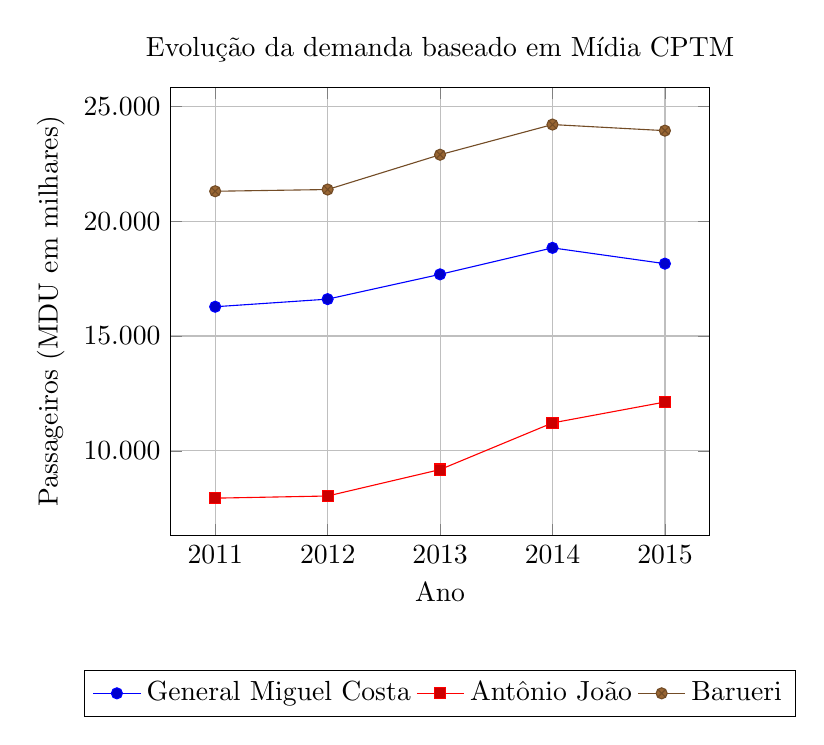
\begin{tikzpicture}
		\begin{axis}[
		title=Evolução da demanda baseado em Mídia CPTM,
		grid=both,
		scaled ticks=false, tick label style={/pgf/number format/fixed},
		x tick label style={/pgf/number format/1000 sep=},
		y tick label style={/pgf/number format/.cd, set thousands separator={.}},
		legend style={at={(0.5,-0.3)},anchor=north,legend columns=-1},
		ylabel=Passageiros (MDU em milhares),
		xlabel=Ano,
		]
		\addplot coordinates
		{(2011,16275) (2012,16606) (2013,17685) (2014,18838) (2015,18150)};
		\addlegendentry{General Miguel Costa}
		
		\addplot coordinates
		{(2011,7943) (2012,8037) (2013,9187) (2014,11218) (2015,12127)};
		\addlegendentry{Antônio João}	
		
		\addplot coordinates
		{(2011,21302) (2012,21377) (2013,22892) (2014,24205) (2015,23940)};
		\addlegendentry{Barueri}
		
		\end{axis}
		\end{tikzpicture}
	\end{center}

%
%==============================================================================================	
%

	\section{Linha 9-Esmeralda: gentrificação}
	
	\begin{wrapfigure}{l}{0.25\textwidth}
		\includegraphics[width=0.9\linewidth]{fotos/20160128_170648.jpg}
		\caption{Mapa da Linha 9 na Estação Berrini (2016)}
	\end{wrapfigure}
	
	\citeonline[pág. 13]{Ferreira} explica que a partir dos anos 1970 o setor industrial localizado no centro metropolitano perdeu importância, de forma que o setor terciário, muito menos concentrado e homogêneo no território, absorveu sua mão de obra, o que se traduz em menor polarização, novas localizações (o autor cita shoppings centers e centros empresariais, por exemplo) e alterações significativas no uso do solo \apud[pág. 25]{Ferreira}{Mello}, o que pode ser relacionado com o processo de rentismo urbano sublinhado por \citeonline[pág 30, nota de rodapé 2]{Acselrad}, no qual ocorre gentrificação estratégica de áreas urbanas outrora industrializadas e marcadas pelo desinvestimento. A gentrificação se dá a partir das possibilidades econômicas, tanto para valorização, como para aquisição de propriedades imobiliária, num processo que exclui moradores de menor renda \apud[pág. 28-29]{Acselrad}{Arantes}. O trecho central da Linha 9-Esmeralda, que avança ao longo da Avenida das Nações Unidas por regiões enobrecidas e substancialmente modificadas pelo processo, é emblemático, não pode por se encaixar no fenômeno que acaba de ser descrito, como também pela extensão do território afetado, que pode ser observado utilizando as estações da CPTM como referência, visto que não há, exceto pela Linha 4-Amarela da \gls{cmsp} em regime de concessão patrocinada, outra infraestrutura de transporte de alta capacidade. As estações são: Hebraica-Rebouças, Cidade Jardim, Vila Olímpia, Berrini e Morumbi.
	
	\begin{figure}[h]
		\caption{Visão dos empreendimentos imobiliários a partir da plataforma da Estação Cidade Jardim (2013}
		\includegraphics[keepaspectratio,width=\textwidth]{fotos/DSCN2007.JPG}
	\end{figure}
	
	\begin{figure}[h]
		\caption{A Estação Cidade Jardim é vizinha de um dos edifícios residenciais mais caros da capital paulista (2013)\cite{apecaro}}
		\includegraphics[keepaspectratio,width=\textwidth]{fotos/DSCN2000.JPG}
	\end{figure}	
	
	\citeonline[pág. 201]{Frugoli} destaca a pressão e o desejo de um ator ligado à iniciativa privada com relação à Linha 9, ainda antes do término de sua dinamização, que resultou, sobretudo, na construção e inauguração das estações Hebraica-Rebouças, Cidade Jardim, Berrini, Morumbi, Granja Julieta, Socorro e Vila Olímpia\cite[pág. 38]{Ferreira}: ``"-- A linha de metrô está pronta. Está aí no Rio Pinheiros, a linha de trem. Não sei por que, até agora, as nossas "autoridades"\dots Eu acho que os caras não têm visão nenhuma, é uma coisa impressionante. É só fazer algumas estações e está pronta. Não, eles vão fazer, mas só quando fizerem a da Rebouças. Faz já! (Entrevista com Carlos Bratke, cit.)''.
	
	Carlos Bratke, como explica \citeonline{Frugoli}. exibe perfeitamente os efeitos descritos por \citeonline{Acselrad}. criticando o poder público, ao mesmo tempo que também demonstra que não era incomodado pela prefeitura ou pelo governo estadual, atuando livremente na Avenida Engenheiro Luís Carlos Berrini:
	
	\begin{citacao}
		As declarações dos irmãos Bratke e matérias da grande imprensa ao longo das últimas décadas ajudam a tecer um quadro que frisa um caráter de "pioneirismo" e "autonomia" quanto ao poder público:
		
		\begin{citacao}
			No espaço de dez anos, [Carlos Bratke, Roberto Bratke e Francisco Collet] operaram em volta da Avenida Luiz Carlos Berrini, sem a mais remota interferência da prefeitura ou de qualquer poder público, uma pequena revolução urbana -- a mais notável já feita num grande espaço da cidade por um único projeto privado de arquitetura. (Veja SP, 1985:16)
		\end{citacao}
		
		Na mesma matéria, Carlos Bratke afirma: "Nunca fui procurado por nenhum órgão público para saber quais são os meus planos" (Veja SP, 1985:21).

		\begin{citacao}		
			"Essa avenida não é um planejamento urbano. Precisavam fazer um canal, então fizeram essa avenida que ligava nada a coisa nenhuma [\dots] Nessa avenida era tudo abandonado, um brejo. Saímos de pastinha na mão, visitando os amigos e convencendo-os a aplicarem o dinheiro no nosso projeto. Falamos com mais de 200 pessoas e tomei muito chá de cadeira que conseguimos construir o primeiro prédio comercial. Arborizamos a região e valorizamos o metro quadrado de 200 para 5 mil dólares. Já fizemos 30. Estamos fazendo mais trinta. (apud Gabaglia, 1990:s.p.)
		\end{citacao}
		
		Outras críticas ao poder público foram coletadas na entrevista que concedeu:
		
		\begin{citacao}
			-- Eu acho que a cidade de São Paulo está constituindo espontaneamente o que os administradores já deviam ter feito há muito tempo: dividir a cidade em vários pólos! [\dots] O zoneamento aqui[região da Berrini] é a coisa mais absurda, anacrônica e idiota que pode existir, mas está acontecendo praticamente numa outra regulamentação. Infelizmente, porque o zoneamento, que já nasceu errado, acabou indo parar nas mãos dos vereadores e não de uma comissão técnica de revisão, nunca foi revisto de uma maneira global, e tem sido alterado ao sabor dos interesses "políticos" dos vereadores. (Entrevista com Carlos Bratke, cit.)
		\end{citacao}
		
	\end{citacao}
	
	\begin{figure}[h]
		\caption{Visão dos empreendimentos imobiliários a partir da plataforma da Estação Berrini (2016)}
		\includegraphics[keepaspectratio,width=\textwidth]{fotos/20160128_170544_HDR.jpg}
	\end{figure}
	
	O Trem Metropolitano, no caso da Linha 9-Esmeralda é interessante por dialogar tanto com a Berrini, como outras avenidas similares (em termos de ocupação do solo), como a Chucri Zaidan (Estação Morumbi) ou ainda, conjuntos de ruas e avenidas, como Funchal, Olimpíadas e Dr. Cardoso de Melo (Estação Vila Olímpia), as sete estações do miolo da Linha 9-Esmeralda,todas já mencionadas anteriormente, foram projetadas por Luiz Carlos Esteves, a respeito delas, destaco numa notícia de 22 de junho de 1998 os seguintes fragmentos:
	
	\begin{citacao}
		Até o final de setembro, a população que freqüenta alguns dos edifícios comerciais mais modernos da cidade, situados na avenida das Nações Unidas, zona sul paulistana, vai passar a contar com uma opção de transporte coletivo. Trata-se das sete novas estações de trem que a CPTM (Companhia Paulista de Trens Metropolitanos) está instalando entre as estações Pinheiros e Largo 13, pertencentes à linha C, que liga Osasco a Jurubatuba.
	
		(\dots)
	
		Luiz Esteves, arquiteto da Harza Hidrobrasileira Engenharia e Projetos, empresa responsável pela concepção e projetos de dinamização da linha Sul, aponta a segurança do usuário como um dos pontos de maior importância das novas estações. “Colocamos a área de bilheteria e catracas junto da calçada dos prédios. Dessa forma, a passarela que leva à plataforma de embarque, do outro lado da marginal, se torna uma área pagante, o que inibe a ação de delinqüentes”, explica.
	
		Outro fator que norteou o projeto, segundo Esteves, foi o urbanismo da região. “Evitamos interferir com o landscape da avenida, projetando estruturas leves e transparentes.” Componentes metálicos fechados com vidro e brises de alumínio garantiram a leveza necessária. O concreto aparece apenas em alguns momentos da estrutura, como a caixa onde serão instaladas duas escadas rolantes, uma escada fixa e um elevador para deficientes. A passarela sobre a marginal também será construída em metal, na forma de uma elipse.
		\cite{trembom}
	\end{citacao}
	
	Na altura, o investimento mencionado foi de US\$ 220 milhões, além disso, Esteves também deu detalhes das estações, então uma novidade. Por se tratar de uma notícia produzida por um periódico especializado em arquitetura, é interessante observarmos que os edifícios da região são enaltecidos ainda antes de introduzir detalhes do investimento feito pelo poder público, a partir daí, vale mencionar que, conforme \cite{Nobre}:
	
	Conforme \citeonline[pág. 145]{Nobre} a ``associação de promotores imobiliários e investidores corporativos, principalmente os fundos de pensão, permitiu a captação de excedentes de capitais e de poupança que puderam ser desviados para a promoção imobiliária dos megaempreendimentos, criando um grande crescimento desse setor do mercado.''\apud{Nobre}{Rolnik}, sendo ainda explicado que a maioria dos empreendimentos ficaram concentrados no Setor Sudoeste da capital paulista em função da estrutura urbana segregada da cidade.
	
	\subsection{Alguns dados}
		
	Conforme dados do \citeonline{ibgeXSP}, São Paulo tem uma população de 11.253.503 habitantes e possui um território com 1.521.110 km$^2$, atendido por 46 estações\cite{sitecptm1}, das quais 5 foram tratadas aqui (10,9\% do total de estações da \gls{cptm} no município), ainda que de forma mais indireta, principalmente em comparação com a subseção sobre a Linha 8-Diamante.
	
	\begin{center}
		\begin{longtable}{|p{1.5cm}|p{2cm}|l|l|l|l|}
			\caption{Demanda do grupo de estações da Linha 9\, baseado em Mídia CPTM}\\
			\hline
			\textbf{Média} & \textbf{Hebraica-Rebouças} & \textbf{Cidade Jardim} & \textbf{Vila Olímpia} & \textbf{Berrini} & \textbf{Morumbi} \\
			\hline
			\endfirsthead
			\multicolumn{3}{c}%
			{\tablename\ \thetable\ -- \textit{Continuado da página anterior}} \\
			\hline
			\textbf{Média} & \textbf{Mooca} & \textbf{Ipiranga} & \textbf{Tamanduateí} \\
			\hline
			\endhead
			\hline \multicolumn{3}{r}{\textit{Continua na próxima página}} \\
			\endfoot
			\hline
			\endlastfoot
			2011 & 18.564 & 16.871 & 25.963 & 20.225 & 20.691 \\
			2012 & 16.363 & 16.891 & 31.733 & 22.893 & 23.105 \\
			2013 & 16.340 & 16.599 & 30.718 & 25.133 & 26.369 \\
			2014 & 16.507 & 15.639 & 32.192 & 25.361 & 28.463 \\
			2015 & 15.872 & 14.820 & 31.130 & 24.238 & 28.048 \\
		\end{longtable}
	\end{center}
	
	\begin{center}
	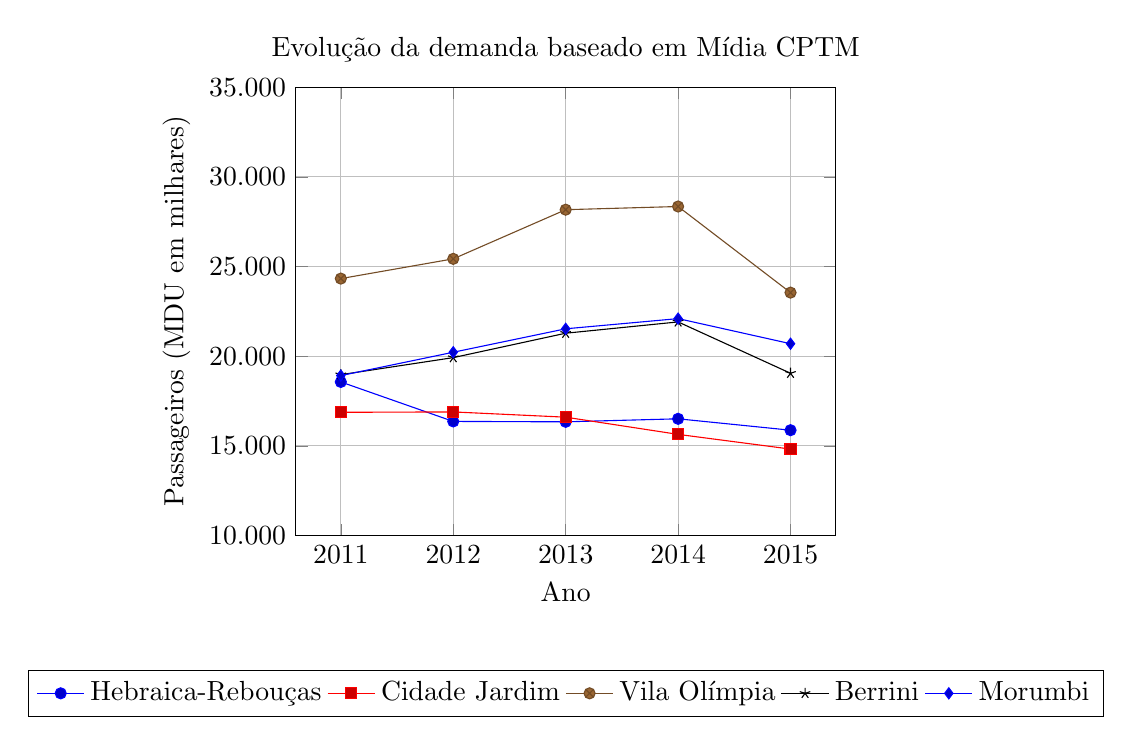
\begin{tikzpicture}
		\begin{axis}[
		title=Evolução da demanda baseado em Mídia CPTM,
		grid=both,
		ymin=10000,
		ymax=35000,
		scaled ticks=false, tick label style={/pgf/number format/fixed},
		x tick label style={/pgf/number format/1000 sep=},
		y tick label style={/pgf/number format/.cd, set thousands separator={.}},
		legend style={at={(0.5,-0.3)},anchor=north,legend columns=-1},
		ylabel=Passageiros (MDU em milhares),
		xlabel=Ano,
		]
		\addplot coordinates
			{(2011,18564) (2012,16363) (2013,16340) (2014,16508) (2015,15873)};
		\addlegendentry{Hebraica-Rebouças}
		
		\addplot coordinates
			{(2011,16871) (2012,16892) (2013,16599) (2014,15640) (2015,14820)};
		\addlegendentry{Cidade Jardim}	
		
		\addplot coordinates
			{(2011,24327) (2012,25428) (2013,28169) (2014,28347) (2015,23545)};
		\addlegendentry{Vila Olímpia}
		
		\addplot coordinates
			{(2011,18968) (2012,19920) (2013,21281) (2014,21911) (2015,19048)};
		\addlegendentry{Berrini}
		
		\addplot coordinates
			{(2011,18918) (2012,20220) (2013,21527) (2014,22096) (2015,20696)};
		\addlegendentry{Morumbi}

		\end{axis}
	\end{tikzpicture}
	\end{center}
	
%
%==============================================================================================	
%
	\section{Linha 10-Turquesa: desindustrialização}
	
	A Linha 10 conecta subcentros regionais que atraem grande interesse para viagens, uma vez que concentram empregos e serviços, atraindo não só a população das cidades atendidas, como Mauá, Santo André e São Caetano, mas também da própria capital, São Paulo\cite[pág. 66]{Ferreira}. Como explica \citeonline[pág. 115]{Stefani}: ``Ocorre aqui, uma situação interessante no processo de industrialização paulista. Apesar de ser o sistema rodoviário, instalado no ABC paulista, o responsável pela implantação de diversos setores industriais em São Paulo, como o de mecânica, metalurgia, elétrica e química, tais setores continuam ainda a se 	instalar no eixo ferroviário e, de certa forma, determinar o crescimento da cidade'', contudo, o mesmo processo não se sustentou em São Paulo, o que se traduz na subutilização do solo urbano ao longo da orla ferroviária após a divisa São Caetano-São Paulo.
	
	\begin{figure}[h]
		\caption{Mapa da rede afixado dentro de um trem da \gls{cmsp}, com parte da Linha 10 visível, de Brás até Utinga (2015)}
		\includegraphics[keepaspectratio,width=\textwidth]{fotos/DSCN5732.JPG}
	\end{figure}
	
	As metrópoles são o palco em que se dão os movimentos de rearranjo das atividades produtivas deprimidas pela suplantação do fordismo e pela desterritorialização/desindustrialização de corte neoliberal\apud{Acselrad}{Veltz}. A Linha 10 da \gls{cptm} é um espelho do impacto dos movimentos mencionados, sendo visíveis as glebas industriais subutilizadas ao longo das Estações Tamanduateí, Ipiranga e Mooca. estações utilizadas aqui para definição do caso da Linha 10.
	
	\begin{figure}[h]
		\caption{Estação Mooca (2016)}
		\includegraphics[width = \textwidth]{fotos/IMG_20160317_165438b.jpg}
	\end{figure}
	
	A visibilidade que menciono no parágrafo anterior é um indicador do descolamento entre uma ferrovia metropolitana com alta capacidade de transporte de passageiros e a orla ferroviária, visto que o acesso às estações acaba sendo prejudicado, bem como seu diálogo com as pessoas, imóveis e equipamentos públicos e privados ao redor. No fragmento abaixo, \citeonline{Acselrad} fornece uma explanação que ajuda a compreender tal descolamento:
	
	\begin{citacao}
		Em contexto de acumulação flexível, a intensificação e variabilidade temporal do uso de recursos ambientais ameaça a estabilidade do “metabolismo urbano”. Conforme sublinha Veltz, a metrópole acelera a divisão do trabalho e a diversificação contínua dos bens e serviços, constituindo-se em lugar privilegiado do redesenvolvimento de sistemas produtivos doravante ultradecompostos. A economia da velocidade e da incerteza, associada a uma demanda cada vez menos previsível, destrói e recria em permanência o território social. Dadas as altas taxas de juros que tornam o peso fundiário das operações muito elevado, o urbanismo just-in-time de mercado – aquele protagonizado pelas próprias empresas – tende a ser cada vez menos regulamentar e cada vez mais comandado pelas	lógicas do capital imobiliário \apud[pág. 351]{Acselrad}{Veltz}. Tudo que diz respeito ao ordenamento espacial regulamentar da cidade, inclusive suas dimensões ecológicas, se esvai em ausência de forças de coordenação, que são eventualmente substituídas pela auto-organização da	“governança corporativa”, da parceria privado-privado, ou seja, em parte crescente, pelos próprios capitais em competição.
		\cite[pág. 31]{Acselrad}
	\end{citacao}
	
	\subsection{Bairros do Tamanduateí}

	A região de atendimento da Linha 10 que estou abordando aqui é objeto de uma \gls{ouc} da Prefeitura de São Paulo. A municipalidade tem em andamento a \gls{ouc} Bairros do Tamanduateí. Destaco dois parágrafos da plataforma Gestão Urbana SP que versam sobre a operação:
	
	\begin{citacao}
		A intervenção tem origem nos estudos da Operação Urbana Diagonal Sul, prevista no Plano Diretor Estratégico de 2002, complementados em 2011 por um Consórcio de empresas capitaneadas pelo escritório Vigliecca e Associados, sob contrato da SMDU. Os estudos então desenvolvidos compreenderam o Plano Urbanístico Específico, o Estudo de Capacidade de Suporte da Infraestrutura de Mobilidade, o Estudo de Avaliação Econômica, o Plano de Comunicação, o Estudo de Impacto Ambiental e o respectivo Relatório de Impacto Ambiental.
	
		Confirmada pelo novo Plano Diretor Estratégico, aprovado pela Lei 16.050 de 31 de julho de 2014, a OUC Bairros do Tamanduateí abrange quase a totalidade do Arco Tamanduateí, um dos Setores da Orla Ferroviária e Fluvial da Macroárea de Estruturação Metropolitana.
		\cite{smdu}
	\end{citacao}
	
	Devido ao passado da linha, sua vocação como via de escoamento de carga e de transporte de mão de obra operária continua mostrando sinais que sobrevivem até os dias atuais. Na capital, as glebas industriais há muito perderam força, dando início a discussões sobre o que fazer em bairros como a Vila Carioca (distrito da Moóca), as quais continuam reacendendo a questão da CPTM, que inclusive chegou a contratar um estudo junto ao UNA Arquitetos para o eixo Moóca-Ipiranga, para o qual:
	
	\begin{citacao}
		Diante da nova inscrição territorial e mudança qualitativa da indústria em São Paulo, o destino de algumas áreas centrais na cidade se tornou objeto urgente de estudo por parte do poder público. A questão é comum à extensão das linhas férreas e coincide com o seu processo de modernização.
		
		O setor Mooca e Ipiranga, cortado pela Avenida do Estado, poderá ser reestruturado a partir desses enormes terrenos vagos. Esses vazios permitem uma nova ocupação que aproxima a população de redes infra-estruturais instaladas. Ao mesmo tempo esses espaços residuais concentram estratos diversos de formação da cidade que merecem ser preservados. O projeto se coloca em sentido de continuidade com os diferentes fluxos da cidade existente, propondo um processo de acumulação de vários tempos em um mesmo espaço. Em contraposição a uma ocupação imobiliária em curso, que segrega e apaga esses vestígios.
		\cite{unaarq}
	\end{citacao}
	
	Legalmente, para que a \gls{ouc} fosse possível, o poder público local da capital definiu o Arco Tamanduateí, o qual está incluído na Macroárea de Estruturação Metropolitana. Fora da macroárea não é possível desenvolver uma operação urbana, que no caso do Arco Tamanduateí, é considerado pela \gls{smdu} um dos principais instrumentos de transformação\cite{smdumacro}.

	\begin{figure}[h]
		\caption{Estação Tamanduateí (2016)}
		\includegraphics[keepaspectratio,width=\textwidth]{fotos/DSCN7465.JPG}
	\end{figure}
	
	A Estação Tamanduateí é, até o momento da produção deste trabalho, a mais moderna de toda a Linha 10-Turquesa, representando avanços drásticos em relação àquelas que estão localizadas no Grande ABC, principalmente. Trata-se de uma estação intermodal, com conexão à Linha 2-Verde do Metrô, além de acesso a ônibus municipais e intermunicipais. Sua construção, no entanto, não representou alterações significativas na região em que se insere, assim, além dos ônibus, sua articulação com o entorno se limita sobretudo ao acesso facilitado a um centro comercial vizinho (Central Plaza Shopping) de uma das faces da estação. Assim como as estações Mooca e Ipiranga, ela está inserida no Arco Tamanduateí e, por conseguinte, na \gls{ouc} Bairros do Tamanduateí.

%	\begin{minipage}[t]{0.5 \linewidth}
	\begin{center}
		\begin{longtable}{|l|l|p{5.3cm}|p{4.5cm}|}
			\caption{Tabela com as linhas de ônibus na Estação Tamanduateí}\\
			\hline
			\textbf{Linha} & \textbf{Tipo} & \textbf{Viagem de Ida} & \textbf{Viagem de Volta} \\
			\hline
			\endfirsthead
			\multicolumn{4}{c}%
			{\tablename\ \thetable\ -- \textit{Continuado da página anterior}} \\
			\hline
			\textbf{Linha} & \textbf{Tipo} & \textbf{Viagem de Ida} & \textbf{Viagem de Volta} \\
			\hline
			\endhead
			\hline \multicolumn{4}{r}{\textit{Continua na próxima página}} \\
			\endfoot
			\hline
			\endlastfoot
			045 & EMTU & Santo André (Vila Palmares) & São Paulo (Tamanduateí) \\
			3134-10 & SPTrans & Shopping Aricanduva & Metrô Tamanduateí \\
			4031-10 & SPTrans & Pq. Santa Madalena & Metrô Tamanduateí \\
			5110-41 & SPTrans & São Mateus & Metrô Tamanduateí \\
			%\hline
		\end{longtable}
	\end{center}
%	\end{minipage}
	
	Segundo informações da plataforma de transparência ``PlanejaSampa'' da Prefeitura de São Paulo, a Meta 123 do Programa de Metas 2013-2016 é a responsável por ``Aprovar a Operação Urbana Bairros do Tamanduateí, a revisão da Operação Urbana Água Branca e iniciar os estudos do projeto Arco Tietê'', tendo sido, conforme dados de 17/12/2015, marcada como concluída, com 100\% dos objetivos atingidos\cite{smg123}.
	
	Amparando-se no \gls{pl} nº 723/2015, que estabelece ``objetivos, diretrizes, estratégias e mecanismos para a implantação da Operação Urbana Consorciada Bairros do Tamanduateí, define Projeto de Intervenção Urbana para a área da Operação Urbana Consorciada e autoriza a criação da empresa Bairros do Tamanduateí S/A''\cite{pl723}, a \gls{smdu} resumidamente determina as seguintes premissas para a \gls{ouc}\cite{smdu2014}:
	
	\begin{itemize}
		\item Cidade compacta: moradia e emprego próximos
		\item Áreas verdes acessíveis numa caminhada de 15 minutos
		\item Uso misto nos imóveis, com fachadas ativas
		\item Integração tipológica, garantindo convivência entre o tecido atual e novas edificações
		\item Maior mobilidade e maior qualidade urbana
	\end{itemize}
	
	Concluindo, as intervenções propostas são faseadas e devem se estender por cerca de 50 anos até elevar as unidades residenciais para 83.958 (estoque de 3.964.499 m$^2$), os leitos hospitalares para 1.540 (ante 366), creches/pré-escolas para 101 (ante 34) e as escolas de ensino fundamental e médio para 45 (ante 22), além disso, o plano prevê um aumento de 138\% de áreas verdes (6 novos parques), além de outras ações ligadas ao viário e drenagem\cite{smdu2014}.
	
	\begin{figure}[h]
		\caption{Cenário temporal 2046: situação final \cite{smdu2014}}
		\includegraphics[keepaspectratio,width=\textwidth]{oucbt_consolidado.png}
	\end{figure}
	
	\subsection{Alguns dados}
	
	Conforme dados do \citeonline{ibgeXSP}, São Paulo tem uma população de 11.253.503 habitantes e possui um território com 1.521.110 km$^2$, atendido por 46 estações\cite{sitecptm1}, das quais 3 foram mencionadas aqui (6,5\% do total de estações da \gls{cptm} no município).
	
	As estações Mooca e Ipiranga possuem um perfil de demanda bastante distinto de Tamanduateí, não sendo nós intermodais, uma vez que não contam com quaisquer facilidades para conexão com ônibus ou, num sentido de maior peso, conexão com outra linha de alta capacidade, como a Linha 2-Verde, acessível por meio da Estação Tamanduateí. A diferença no perfil de demanda exigiu a separação da Estação Tamanduateí no gráfico que veremos a seguir.
	
	\begin{center}
		\begin{longtable}{|p{2cm}|p{3cm}|p{3cm}|p{3cm}|}
			\caption{Demanda do grupo de estações da Linha 10\, baseado em Mídia CPTM}\\
			\hline
			\textbf{Média} & \textbf{Mooca} & \textbf{Ipiranga} & \textbf{Tamanduateí} \\
			\hline
			\endfirsthead
			\multicolumn{3}{c}%
			{\tablename\ \thetable\ -- \textit{Continuado da página anterior}} \\
			\hline
			\textbf{Média} & \textbf{Mooca} & \textbf{Ipiranga} & \textbf{Tamanduateí} \\
			\hline
			\endhead
			\hline \multicolumn{3}{r}{\textit{Continua na próxima página}} \\
			\endfoot
			\hline
			\endlastfoot
			2011 & 7.689 & 10.900 & 45.971 \\
			2012 & 8.072 & 10.578 & 53.779 \\
			2013 & 7.950 & 10.620 & 58.093 \\
			2014 & 7.664 & 10.558 & 58.112 \\
			2015 & 6.872 & 9.505 & 57.864 \\
		\end{longtable}
	\end{center}

	\newpage
	
	\begin{center}
		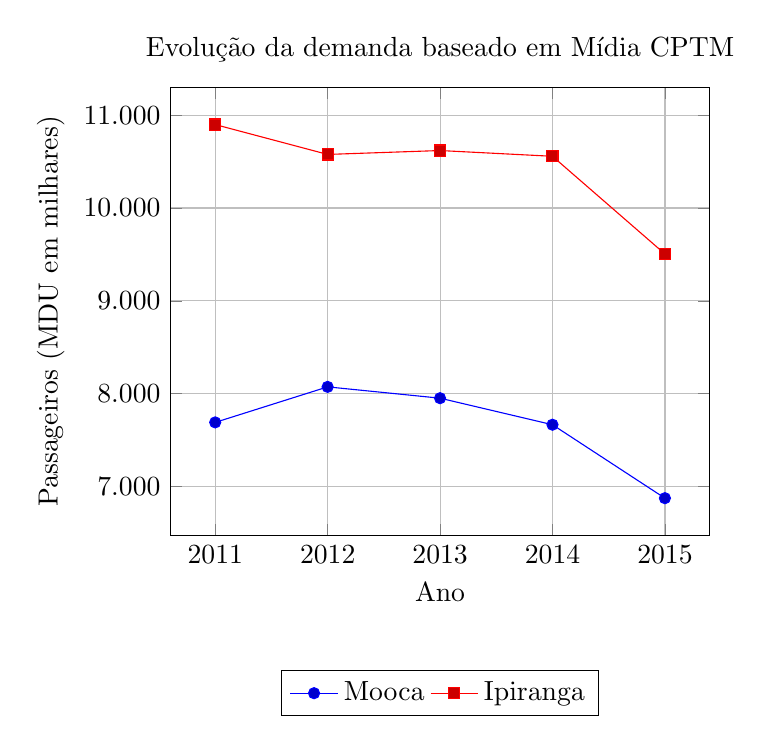
\begin{tikzpicture}
		\begin{axis}[
		title=Evolução da demanda baseado em Mídia CPTM,
		grid=both,
		scaled ticks=false, tick label style={/pgf/number format/fixed},
		x tick label style={/pgf/number format/1000 sep=},
		y tick label style={/pgf/number format/.cd, set thousands separator={.}},
		legend style={at={(0.5,-0.3)},anchor=north,legend columns=-1},
		ylabel=Passageiros (MDU em milhares),
		xlabel=Ano,
		]
		\addplot coordinates
		{(2011,7689
			) (2012,8072) (2013,7950) (2014,7664) (2015,6872)};
		\addlegendentry{Mooca}
		
		\addplot coordinates
		{(2011,10900) (2012,10578) (2013,10620) (2014,10558) (2015,9505)};
		\addlegendentry{Ipiranga}
				
		\end{axis}
		\end{tikzpicture}
	\end{center}
	
	A demanda da Estação Tamanduateí, já em 2011, superava 40 mil passageiros em \gls{mdu}, número que é superior ao de todas as estações abordadas neste trabalho.

	\begin{center}
		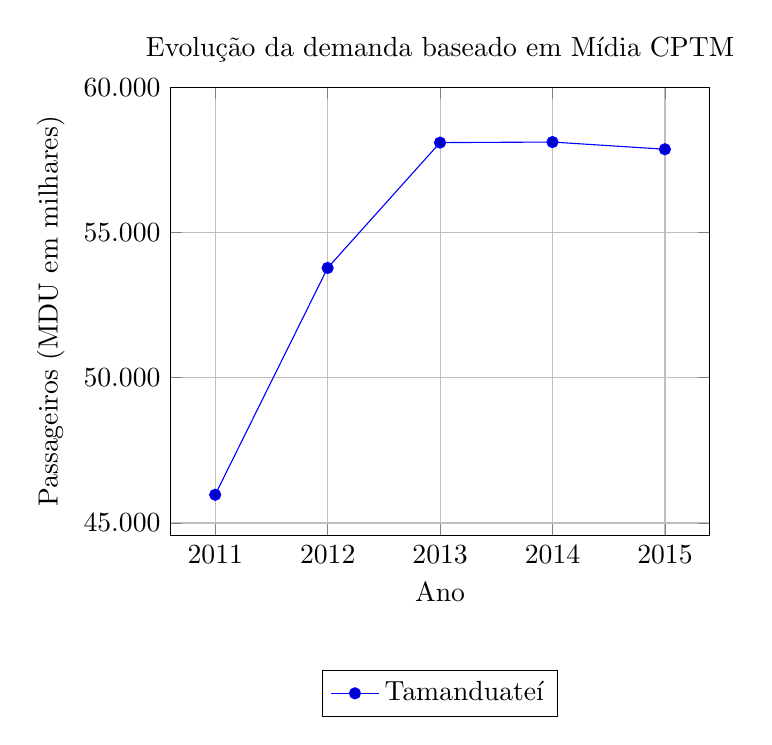
\begin{tikzpicture}
		\begin{axis}[
		title=Evolução da demanda baseado em Mídia CPTM,
		grid=both,
		ymax=60000,
		x tick label style={/pgf/number format/1000 sep=},
		y tick label style={/pgf/number format/.cd, set thousands separator={.}},
		legend style={at={(0.5,-0.3)},anchor=north,legend columns=-1},
		scaled ticks=false, tick label style={/pgf/number format/fixed},
		ylabel=Passageiros (MDU em milhares),
		xlabel=Ano,
		]
		\addplot coordinates
		{(2011,45971) (2012,53779) (2013,58093) (2014,58112) (2015,57864)};
		\addlegendentry{Tamanduateí}
		
		\end{axis}
		\end{tikzpicture}
	\end{center}

%
%==============================================================================================	
%

	\chapter{Conclusão}
	
	O presente trabalho permitiu ``costurar'' melhor alguns conceitos apresentados pela disciplina, de forma a garantir sua fixação com a aplicação dos conceitos em situações presentes em parte da área de influência da infraestrutura de transporte sobre trilhos da {\glsdesc*{cptm}}. Foi possível estabelecer relações para além da bibliografia básica, mas sempre mantendo a transversalidade.
	
	É flagrante a necessidade de estruturar melhores políticas públicas que recuperem, em totalidade, o potencial estruturante da ferrovia, ao mesmo tempo que garantam a sobrevivência das mesmas políticas com base na infraestrutura que lhes servirá de justificativa em primeiro lugar.
	
	Fica também evidente a heterogeneidade não só da capital ou da \gls{rmsp}, mas da própria malha do Trem Metropolitano, o que se deve, como vimos, a heranças de estatais diferentes, cada qual com seu contexto histórico particular.
	
	% ----------------------------------------------------------
	% ----------------------------------------------------------
	\postextual
	
	
	
	% informa o arquivo com a bibliografia. Deve ser o mesmo nome
	% (sem o sufixo) que será informado no ambiente filecontents
	% que está no final deste arquivo. Neste exemplo foi usado 
	% bibitemp.bib e bibtemp. Este comando insere a bibliografia
	% nesta posição (antes dos apêndices, anexos, índice remissivo)
	\bibliography{referencias}
	% ----------------------------------------------------------
	% Glossário
	% ----------------------------------------------------------
	% Consultar manual da classe abntex2 para orientações sobre o
	% uso do glossário.
	\renewcommand{\glossaryname}{Glossário}
	%\renewcommand{\glossarypreamble}{Esta é a descrição do glossário.\\ \\}
	\renewcommand*{\glsseeformat}[3][\seename]{\textit{#1}
	\glsseelist{#2}}

	% ---
	% Traduções para o ambiente glossaries
	% ---
	\providetranslation{Glossary}{Glossário}
	\providetranslation{Acronyms}{Siglas}
	\providetranslation{Notation (glossaries)}{Notação}
	\providetranslation{Description (glossaries)}{Descrição}
	\providetranslation{Symbol (glossaries)}{Símbolo}
	\providetranslation{Page List (glossaries)}{Lista de Páginas}
	\providetranslation{Symbols (glossaries)}{Símbolos}
	\providetranslation{Numbers (glossaries)}{Números} 
	% ---
	
	% ---
	% Imprime o glossário
	% ---
	\cleardoublepage
	\phantomsection
	\addcontentsline{toc}{chapter}{\glossaryname}
	% \glossarystyle{index}
	% \glossarystyle{altlisthypergroup}
	\glossarystyle{tree}
	\printglossaries
	% ---
	
	% ----------------------------------------------------------
	% Apêndices
	% ----------------------------------------------------------
	
	% ---
	% Inicia os apêndices. Não esquecer de fechar ao final de
	% todos os apêndices (\end{apendicesenv})
	% ---
	%\begin{apendicesenv}
	
	% Imprime uma página indicando o início dos apêndices
	%\partapendices
	
	% ----------------------------------------------------------
	%\chapter{Primeiro apêndice}
	% ----------------------------------------------------------
	
	%Este é um exemplo de inclusão de capítulos de %apêndice em uma 
	%monografia.  Cada apêndice é tratado como se fosse %um capítulo.
	%Os apêndices devem ser iniciados pelo comando de %ambiente
	%\textbackslash begin\{apendicesenv\} e encerrados %pelo comando 
	%\textbackslash end\{apendicesenv\}.
	
	% ----------------------------------------------------------
	%\chapter{Segundo apêndice}
	% ----------------------------------------------------------
	
	%Este é um exemplo de inclusão de um segundo apêndice. 
	
	%\end{apendicesenv}
	% ---
	
	
	% ----------------------------------------------------------
	% Anexos
	% ----------------------------------------------------------
	
	% ---
	% Inicia os anexos
	% ---
	%\begin{anexosenv}
	
	% Imprime uma página indicando o início dos anexos
	%\partanexos
	
	% ---
	%\chapter{Primeiro anexo}
	% ---
	%Os anexos são similares aos apêndices se distinguindo pelo fato
	%que os apêndices são de autoria do autor da monografia e os 
	%anexos não são da autoria do autor da monografia.  Por exemplo,
	%se incluir no trabalho um modelo de um formulário preenchido
	%por alunos participantes de uma pesquisa, este será um apêndice
	%se o formulário foi criado pelo autor da monografia e será um
	%anexo se o formulário tiver sido criado por outros (por exemplo,
	%é um formulário padrão da escola em que o aluno que o preenche
	%estuda).
	%
	%Mesmo que o formulário tenha sido elaborado pela escola, uma
	%reprodução do formulário preenchido por cada aluno na pesquisa
	%será incluído no apêndice pois envolve o trabalho do autor da
	%monografia ao distribuir, coletar e reproduzir as respostas.
	%
	%Este é um exemplo de inclusão de capítulos de anexos em uma 
	%monografia.  Cada anexo é tratado como se fosse um capítulo.
	%Os anexos devem ser iniciados pelo comando de ambiente
	%\textbackslash begin\{anexoenv\} e encerrados pelo comando 
	%\textbackslash end\{anexoenv\}.
	%
	%\end{anexosenv}
	% ---
	%---------------------------------------------------------------------
	%---------------------------------------------------------------------
	
	%\printindex
	
	% Por padrão são incluídas no trabalho somente as referências
	% citadas ao longo do texto. No comando abaixo foram acrescentadas
	% algumas referências não citadas (neste texto servem apenas como
	% exemplos). Não deve ser usado o comando (mais simples) 
	% \nocite{*}, pois este parece não ser compatível com o
	% abntex2cite
	%\nocite{abntex2cite,abntex2wiki,boyer,eves,iezzi,kletenic,
	%        diomara,steinbruch,intusolatex,feynman,shannon,
	%        luisfelipe,turing}
\end{document}
